\section{{Descripción casos de uso}}

%--------------------------Inicia otro caso de uso (javier)--------------------------------------------------------------%

\subsection{\textcolor{blue}{CU 1.1 Restablecer contraseña}}

\subsubsection{\textcolor{blue}{Resumen}}
Se brindara al usuario la posibilidad de recuperar sus datos para acceder al sistenma en caso de haberlos olvidado o perdido.
\subsubsection{\textcolor{blue}{Descripción}}
\begin{tabularx}{16cm}{||l|X||}
	\hline
	\multicolumn{2}{||c||}{Caso de Uso: Reestablecer contraseña } \\
	\hline
	\multicolumn{2}{||c||}{\textcolor{blue}{Resumen de atributos}} \\
	\hline
	{Autor:} & Zamarrón Ramírez Javier \\
    \hline
	{Actor:} & Usuario turista\\
	\hline
	{Próposito:} & Permitir al usuario restablecer contraseña\\
	\hline
	{Entradas:} &  Se escribe desde la pantalla del celular el correo electrónico del usuario. \\
	\hline
	{Salidas:} & Se envía el mensaje de correo electrónico de recuperación de contraseña \\
	\hline
	{Precondiciones:} & Debe existir una cuenta activa en el sistema con el correo electronico.\\ 
	\hline
	{Postcondiciones:} & Se elimina la cuenta del usuario, por lo que el sistema deja de almacenar su informacion.\\
	\hline
	{Errores:} &\begin{minipage}{1\linewidth}
        \begin{enumerate}
            \item Cuando el correo electrónico no es válido, se mostrará el mensaje de alerta 1.
            \item Cuando el correo electrónico no está asociado a una cuenta activa, se mostrará el mensaje de alerta 2.
            \item Cuando las contraseñas no son iguales, se mostrará el mensaje de alerta 3.
            \item Cuando la contraseña no cumple con la regla de negocio 5, se mostrará el mensaje de alerta 4.
        \end{enumerate}
    \end{minipage} \\
	\hline
	{Tipo:} & Reunion interna\\
	\hline
	{Fuente:} & {-} \\
	\hline
	{Observaciones:} & {-} \\
	\hline
\end{tabularx}

\pagebreak
\subsubsection{\textcolor{blue}{Trayectorias del caso de uso}}
\textbf{Trayectoria Principal}
    \begin{enumerate}
    \item 
\includegraphics[width=0.0150\textwidth]{Figuras/persona.png} presiona la leyenda olvidaste tu contraseña? en la pantalla \textcolor{blue}{Iniciar sesion}.
    \item 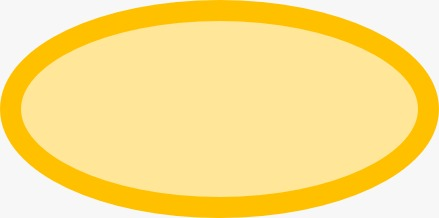
\includegraphics[width=0.0500\textwidth]{Figuras/sistema.png} muestra la pantalla Recuperar contraseña.
    \item 
\includegraphics[width=0.0150\textwidth]{Figuras/persona.png} solicita recuperar los datos de su cuenta oprimiendo ¿Olvidaste tu contraseña? de la pantalla \textcolor{blue}{Iniciar sesion}.
     \item 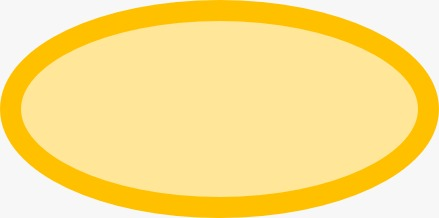
\includegraphics[width=0.0500\textwidth]{Figuras/sistema.png} solicita ingresar el correo electronico asociado a la cuenta de la que se desea reestablecer la contraseña mostrando la pantalla \textcolor{blue}{Recuperacion de contraseña} [Trayectoria A].
    \item 
\includegraphics[width=0.0150\textwidth]{Figuras/persona.png} ingresa el correo electronico .
    \item 
\includegraphics[width=0.0150\textwidth]{Figuras/persona.png} solicita reestablecer la contraseña de su cuenta oprimiendo el boton de enviar correo.
    \item 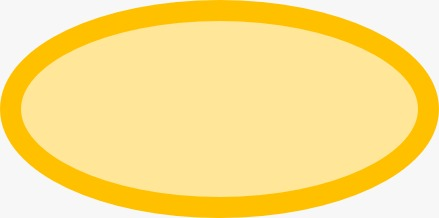
\includegraphics[width=0.0500\textwidth]{Figuras/sistema.png} verifica que el correo electronico sea valido. [Trayectoria B]
    \item 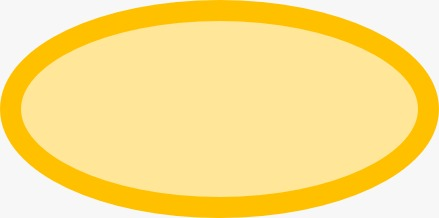
\includegraphics[width=0.0500\textwidth]{Figuras/sistema.png} verifica que el correo electronico este asociado a una cuenta activa. [Trayectoria C].
    \item 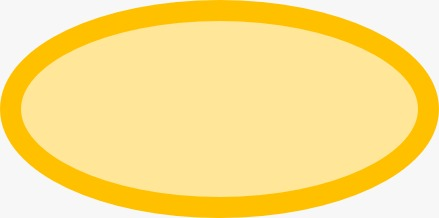
\includegraphics[width=0.0500\textwidth]{Figuras/sistema.png} genera y registra el token de restablecimiento de contraseña.
    \item 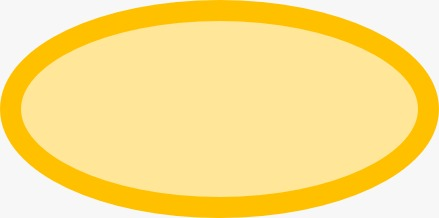
\includegraphics[width=0.0500\textwidth]{Figuras/sistema.png} envia por correo electronico el mensaje \textcolor{blue}{E-mail1 Correo recuperación de contraseña} .
    \item 
\includegraphics[width=0.0150\textwidth]{Figuras/persona.png} accede al enlace enviado por correo electrónico.
    \item 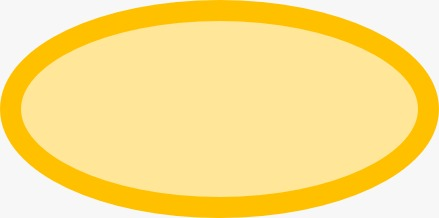
\includegraphics[width=0.0500\textwidth]{Figuras/sistema.png} recibe la solicitud del usuario para restablecer contraseña.
    \item 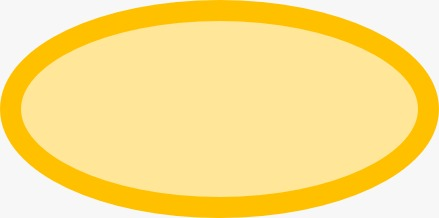
\includegraphics[width=0.0500\textwidth]{Figuras/sistema.png} verifica que el token de la cuenta sea valido.
    \item 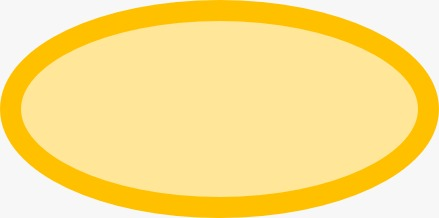
\includegraphics[width=0.0500\textwidth]{Figuras/sistema.png} verifica que el token de la cuenta sea valido.
    \item 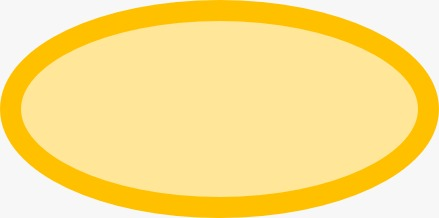
\includegraphics[width=0.0500\textwidth]{Figuras/sistema.png} muestra al usuario la pantalla de Restablecer contraseña.
    \item 
\includegraphics[width=0.0150\textwidth]{Figuras/persona.png} escribe sus contraseñas y presiona el boton Guardar contraseña.
    \item 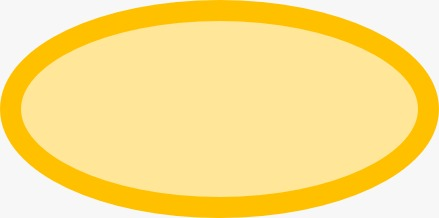
\includegraphics[width=0.0500\textwidth]{Figuras/sistema.png} verifica si ambas contraseñas son iguales. [Trayectoria D]
    \item 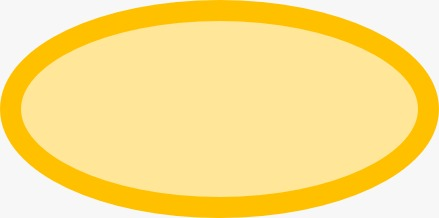
\includegraphics[width=0.0500\textwidth]{Figuras/sistema.png} verifica si la contraseña proporcionada cumple con los requisitos mencionados en la regla de negocio 5. [Trayectoria E]
    \item 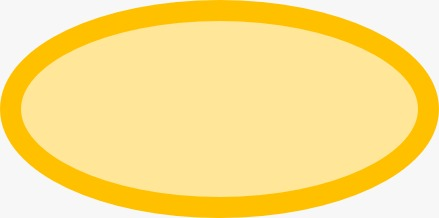
\includegraphics[width=0.0500\textwidth]{Figuras/sistema.png} elimina el token de restablecimiento de contraseña generado.
    \item 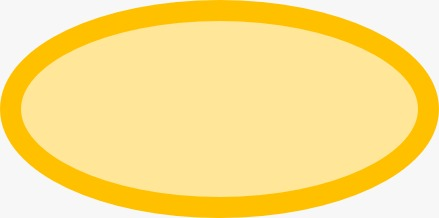
\includegraphics[width=0.0500\textwidth]{Figuras/sistema.png} actualiza la contraseña del usuario.
    \item 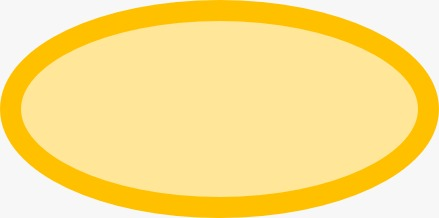
\includegraphics[width=0.0500\textwidth]{Figuras/sistema.png} muestra la pantalla Recuperacion de contraseña (exitoso) y se redirecciona a pantalla Iniciar sesion.\\
    - - - Fin de caso de uso
\end{enumerate}

\textbf{Trayectoria A}\\
Condición : 
\includegraphics[width=0.0150\textwidth]{Figuras/persona.png} desea cancelar el cambio de contraseña
\begin{itemize}
    \item 
\includegraphics[width=0.0150\textwidth]{Figuras/persona.png} oprime el boton de regresar.
     \item 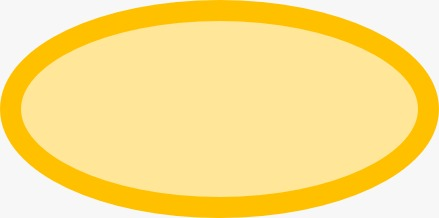
\includegraphics[width=0.0500\textwidth]{Figuras/sistema.png} muestra la pantalla Iniciar sesion.
    \item Termina el caso de uso.\\
    - - - Fin de trayectoria
\end{itemize}
\textbf{Trayectoria B}\\
Condición :  
\includegraphics[width=0.0150\textwidth]{Figuras/persona.png} no escribio un correo valido.
\begin{itemize}
    \item 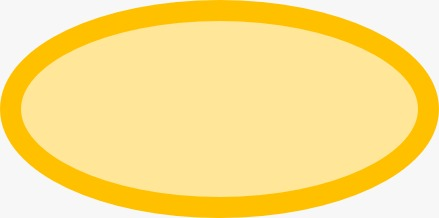
\includegraphics[width=0.0500\textwidth]{Figuras/sistema.png} muestra en la pantalla Recuperacion de contraseña el mensaje alerta 1.
    \item Continua en el paso 5\\
    - - - Fin de trayectoria
\end{itemize}
\textbf{Trayectoria C}\\
Condición : 
\includegraphics[width=0.0150\textwidth]{Figuras/persona.png} escribio un correo electronico que no esta asociado a una cuenta activa.
\begin{itemize}
    \item 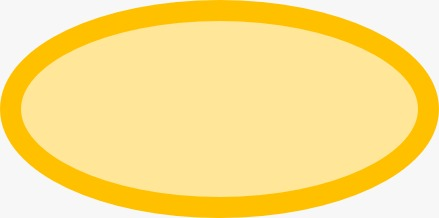
\includegraphics[width=0.0500\textwidth]{Figuras/sistema.png} muestra en la pantalla Recuperacion de contraseña el mensaje alerta 2.
    \item Continua en el paso 3\\
    - - - Fin de trayectoria
\end{itemize}
\textbf{Trayectoria D}\\
Condición : Las contraseñas escritas por 
\includegraphics[width=0.0150\textwidth]{Figuras/persona.png} no son iguales.
\begin{itemize}
    \item  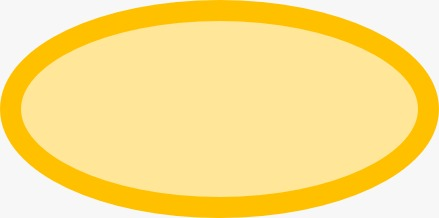
\includegraphics[width=0.0500\textwidth]{Figuras/sistema.png} muestra en la pantalla restablecer contraseña el mensaje alerta 3.
    \item Continua en el paso 14.\\
    - - - Fin de trayectoria
\end{itemize}
\textbf{Trayectoria E}\\
Condición : La contraseña escrita por el 
\includegraphics[width=0.0150\textwidth]{Figuras/persona.png} no cumple con la regla de negocio 5.
\begin{itemize}
    \item 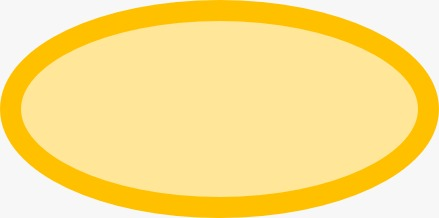
\includegraphics[width=0.0500\textwidth]{Figuras/sistema.png} muestra en la pantalla restablecer contraseña el mensaje alerta 4.
    \item Continua en el paso 14.\\
    - - - Fin de trayectoria
\end{itemize}
\subsubsection{\textcolor{blue}{Pantalla IU3 y IU4}}

    \begin{figure}[htb]
        \centering
        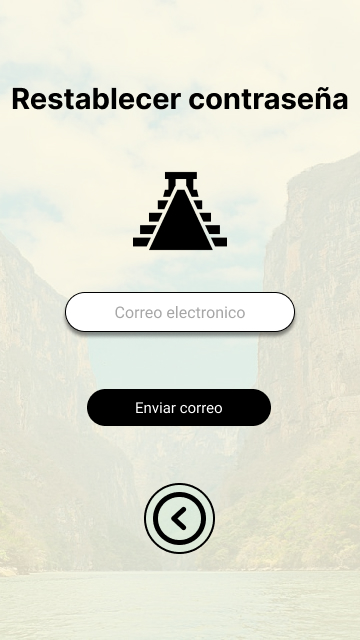
\includegraphics[width= 5cm]{Pantallas Prototipo3/IU03 Pantalla correo restablecimiento.jpg}
        \caption{IU03 Recuprar contraseña}
        \label{fig:enter-label}
    \end{figure}
    \begin{figure}[htb]
        \centering
        \includegraphics[width= 5cm]{Pantallas Prototipo3/IU05-Reestablacer contraseña.jpg}
        \caption{IU04 Escribir contraseña nueva}
        \label{fig:enter-label}
    \end{figure}

%---------------------------------------Finaliza caso de uso (javier)%---------------------------------------------------
%-----------------------------------------------------------------------------------------------------------------------
%--------------------------Inicia otro caso de uso (Dario)--------------------------------------------------------------%
\newpage
\subsection{\textcolor{blue}{CU2.1 Actualizar datos de perfil}}

\subsubsection{\textcolor{blue}{Resumen}}
Se brinda la posibilidad al usuario de modificar sus datos una vez registrado en el sistema, los datos que puede modificar son su nombre, teléfono y su contraseña, para esto debe de comprobar que la cuenta es de su propiedad digitando su contraseña actual.
\subsubsection{\textcolor{blue}{Descripción}}

\begin{tabularx}{16cm}{||l|X||}
	\hline
	\multicolumn{2}{||c||}{Caso de Uso: xxdl} \\
	\hline
	\multicolumn{2}{||c||}{\textcolor{blue}{Resumen de atributos}} \\
 \hline
	{Autor:} & {\textcolor{blue}{Alvarado Dario}} \\
	\hline
	\hline
	{Actor:} & {\textcolor{blue}{Usuario Turista}} \\
	\hline
	{Próposito:} & Permitir al usuario modificar sus datos para mantener su información actualizada.\\
	\hline
	{Entradas:} & {Se escribe desde el teclado el nuevo Nombre del usuario
 Se escribe desde el teclado el nuevo número telefónico del usuario
 Se escribe desde el teclado la nueva contraseña del usuario
 Se escribe desde el teclado la confirmación de la nueva contraseña del usuario
}
        \\
	\hline
	{Salidas:} & {Se mostrará en la pantalla el mensaje MSG Operación exitosa al guardar los cambios.}\\
	\hline
	{Precondiciones:} & {Que la cuenta este activa en el sistema.}\\
    \hline
	{Postcondiciones:} & {Se modifica los datos que el usuario elija de su cuenta.
 Se notifica al usuario sobre la actualización exitosa o cualquier error que haya ocurrido.}\\
	\hline
	{Errores:} & {Cuando el usuario digita mal su contraseña actual se mostrará el MSG contraseña errónea
 Cuando no coincida la contraseña con la confirmación de contraseña, se mostrará el mensaje MSG Coincidencia de contraseña incorrecta
 Cuando la nueva contraseña no tiene el formato correcto se mostrará el mensaje contraseña mal formada
 Cuando no coincida la nueva contraseñan con la confirmación de nueva contraseña, se mostrará el mensaje MSG Coincidencia de contraseña incorrecta
 Cuando el nuevo número telefónico tiene el formato correcto se mostrará el mensaje Número telefónico invalido
 Cuando se requieren modificar los datos de una cuenta inactiva se mostrara el mensaje MSG modificación de datos cuenta inactiva} \\
	\hline
	{Tipo:} & {-}\\
	\hline
	{Fuente:} & {-} \\
	\hline
	{Observaciones:} & {-} \\
	\hline
\end{tabularx}

\subsubsection{\textcolor{blue}{Trayectorias del caso de uso}}

\textbf{Trayectoria Principal}
\begin{enumerate}
    \item 
\includegraphics[width=0.0150\textwidth]{Figuras/persona.png} Solicita actualizar sus datos oprimiendo el botón Actualizar Datos de la pantalla UI Pantalla de perfil.
    \item 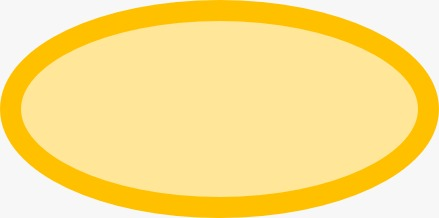
\includegraphics[width=0.0500\textwidth]{Figuras/sistema.png} Presenta la pantalla UI Confirmar contraseña.
    \item 
\includegraphics[width=0.0150\textwidth]{Figuras/persona.png} Ingresa su contraseña actual en un campo designado.
    \item 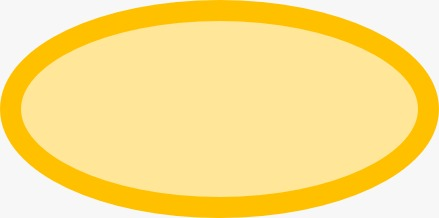
\includegraphics[width=0.0500\textwidth]{Figuras/sistema.png} El sistema verifica si el usuario ha ingresado su contraseña actual para confirmar la autenticidad del cambio [Trayectoria A] [Trayectoria B].
     \item 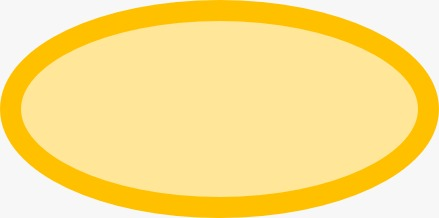
\includegraphics[width=0.0500\textwidth]{Figuras/sistema.png} Presenta una pantalla que muestra los campos para editar el nombre, el teléfono y la contraseña. Cada campo prellenado con la información actual del usuario. 
    \item 
\includegraphics[width=0.0500\textwidth]{Figuras/persona.png} Modifica uno o más de los campos, ya sea el nombre, el teléfono y/o la contraseña, según sus necesidades. [Trayectoria C].
    \item 
\includegraphics[width=0.0500\textwidth]{Figuras/persona.png} Decide guardar los cambios y presiona un botón o enlace de "Guardar" o "Actualizar".
    \item 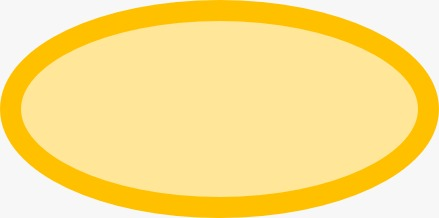
\includegraphics[width=0.0500\textwidth]{Figuras/sistema.png} verifica que se haya ingresado los datos nuevos de manera correcta según la regla de negocio RN Establecimiento de teléfono, [Trayectoria D].
    \item 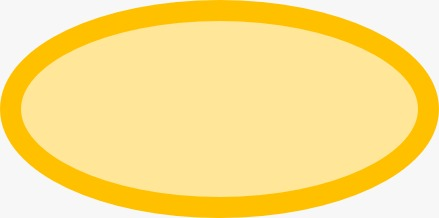
\includegraphics[width=0.0500\textwidth]{Figuras/sistema.png} Muestra la pantalla IU actualización exitosa, indicando que los datos se han actualizado satisfactoriamente.
    \item 
\includegraphics[width=0.0500\textwidth]{Figuras/persona.png} Tiene la opción de regresar a la pantalla principal o continuar realizando otras acciones dentro de la aplicación.
    
\end{enumerate}
\textbf{---Fin del caso de Uso---}
\vspace{15pt}

\textbf{Trayectoria Alternativa A}

Condición: El usuario digita erróneamente su contraseña 

\begin{itemize}
    \item 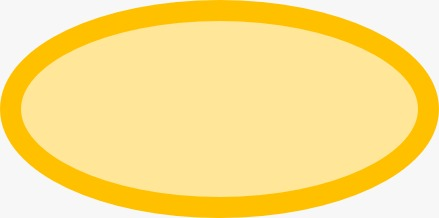
\includegraphics[width=0.0150\textwidth]{Figuras/sistema.png} arroja el mensaje MSJ Contraseña errónea
    \item 
\includegraphics[width=0.01500\textwidth]{Figuras/persona.png} Da clic en el botón Aceptar
  \item 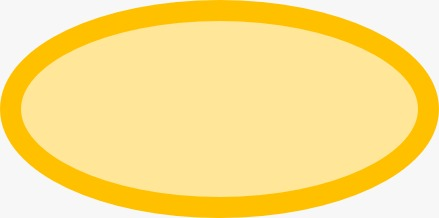
\includegraphics[width=0.0150\textwidth]{Figuras/sistema.png} Muestra la pantalla UI Pantalla de perfil
    
\end{itemize}
---Fin de trayectoria

\vspace{15pt}

\textbf{Trayectoria Alternativa B}

Condición: El usuario da clic en el botón Cancelar
\begin{itemize}
    \item 
\includegraphics[width=0.0150\textwidth]{Figuras/persona.png} Da clic en el botón Cancelar
    \item 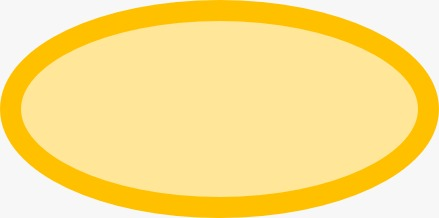
\includegraphics[width=0.01500\textwidth]{Figuras/sistema.png} Muestra la pantalla UI Pantalla de perfil.
\end{itemize}
---Fin de trayectoria

\vspace{15pt}

\textbf{Trayectoria Alternativa C}
Condición: El usuario desea descartar los cambios

\begin{itemize}
    \item 
\includegraphics[width=0.0150\textwidth]{Figuras/persona.png} Oprime el botón Descartar cambios
    \item \includegraphics[width=0.01500\textwidth]{Figuras/sistema.png} Muestra la pantalla IU Descartar cambios.
     \item \includegraphics[width=0.01500\textwidth]{Figuras/sistema.png} Muestra la pantalla IU perfil
\end{itemize}
---Fin de trayectoria
\vspace{15pt}


\textbf{Trayectoria Alternativa D}
Condición: El usuario ingresa de manera errónea un campo

\begin{itemize}
    \item \includegraphics[width=0.0150\textwidth]{Figuras/sistema.png} Muestra el mensaje MSJ Campo teléfono Invalido.
    \item \includegraphics[width=0.01500\textwidth]{Figuras/persona.png} Oprime el botón Aceptar
     \item \includegraphics[width=0.01500\textwidth]{Figuras/sistema.png} Muestra la pantalla UI Actualizar Datos.
\end{itemize}
---Fin de trayectoria
\vspace{15pt}

\textbf{Caso de uso que extienden}

\begin{itemize}
    \item Eliminar cuenta
Condición: El usuario da clic en el botón Eliminar cuenta


    \item Preferencias
Condición: El usuario da clic en el botón Preferencias
   
\end{itemize}
---Fin de trayectoria
\vspace{15pt}


\subsubsection{\textcolor{blue}{Pantalla IU16}}

\textbf{Objetivo} \\
Permitir al usuario el consultar y editar su perfil.
\vspace{15pt}

\textbf{Diseño}

    \begin{figure}[h]
        
            \centering
            \includegraphics[width=.4\linewidth]{Pantallas Prototipo3/IU16 Pantalla de seleccionar el dato a editar.jpg}
            \caption{Pantalla IU16 Seleccionar dato}
    
    \end{figure}


%---------------------------------------Finaliza caso de uso (Dario)%---------------------------------------------------
%-----------------------------------------------------------------------------------------------------------------------

%-----------------------------------------------------------------------------------------------------------------------
%--------------------------Inicia otro caso de uso (said)--------------------------------------------------------------%

\subsection{\textcolor{blue}{CU 2.2 Eliminar cuenta}}

\subsubsection{\textcolor{blue}{Resumen}}
Se brinda al usuario la posibilidad de poder eliminar su cuenta, además se necesita ingresar la contraseña como metodo de validacion.
\subsubsection{\textcolor{blue}{Descripción}}
\begin{tabularx}{16cm}{||l|X||}
	\hline
	\multicolumn{2}{||c||}{Caso de Uso: } \\
	\hline
	\multicolumn{2}{||c||}{\textcolor{blue}{Resumen de atributos}} \\
	\hline
	{Autor:} & Estrada Yepez Omar Said \\
    \hline
	{Actor:} & Usuario turista\\
	\hline
	{Próposito:} & Que el sistema permita al usuario eliminar su cuenta en cualquier momento si asi lo desea.\\
	\hline
	{Entradas:} &  Boton con el nombre de Actualizar datos. \\
    &Se ingresa la contraseña del usuario\\
    &Se ingresa la confirmacion de la contraseña del usuario.\\
    &Boton para validar contraseñas\\
    &Boton de confirmacion de eliminar\\
	\hline
	{Salidas:} & En la pantalla se mostrara el mensaje "Su cuenta fue eliminada con exito"\\
	\hline
	{Precondiciones:} & Debe existir una cuenta activa en el sistema con el correo electronico.\\ 
	\hline
	{Postcondiciones:} & Se elimina la cuenta del usuario, por lo que el sistema deja de almacenar su informacion.\\
	\hline
	{Errores:} & Cuando se proporciona la contraseña no coincide con el formato requerido de una contraseña. \\
    &No coincide la contraseña con la confirmacion de contraseña, se muestra el mensaje Las contraseñas deben ser iguales.\\
	\hline
	{Tipo:} & -\\
	\hline
	{Fuente:} & Reunion interna \\
	\hline
	{Observaciones:} & {-} \\
	\hline
\end{tabularx}

\pagebreak
\subsubsection{\textcolor{blue}{Trayectorias del caso de uso}}
\textbf{Trayectoria Principal}
    \begin{enumerate}
        \item \includegraphics[width=0.0150\textwidth]{Figuras/persona.png} El usuario solicita modificar datos oprimiendo el boton \includegraphics[width=0.2\textwidth]{ComponentesCU/AD.png}  de \textcolor{blue}{IU14 Pantalla de perfil}.
        \item \includegraphics[width=0.0500\textwidth]{Figuras/sistema.png} Muestra \textcolor{blue}{IU16 Pantalla de seleccionar el dato a editar}, mostrando en la parte inferior derecha el boton \includegraphics[width=0.2\textwidth]{ComponentesCU/img.png}.
        \item \includegraphics[width=0.0150\textwidth]{Figuras/persona.png} Oprime el boton \includegraphics[width=0.2\textwidth]{ComponentesCU/img.png}.
         \item \includegraphics[width=0.0500\textwidth]{Figuras/sistema.png} Muestra la \textcolor{blue}{IU15 Validacion de contrasena para modificacion de datos}.
        \item \includegraphics[width=0.0500\textwidth]{Figuras/sistema.png} Solicita la contraseña y confirmacion de contraseña del usuario.
        \item \includegraphics[width=0.0150\textwidth]{Figuras/persona.png} Ingresa su contraseña y su confirmacion de la misma.
        \item \includegraphics[width=0.0500\textwidth]{Figuras/sistema.png} Valida que las contraseñas sean iguales[Trayectoria A].
        \item \includegraphics[width=0.0150\textwidth]{Figuras/persona.png} Oprime el boton \includegraphics[width=0.2\textwidth]{ComponentesCU/img1.png} de \textcolor{blue}{IU15 Validacion de contrasena para modificacion de datos}.
        \item \includegraphics[width=0.0500\textwidth]{Figuras/sistema.png} Muestra l\textcolor{blue}{IU19 Ventana de confirmaci ́on de eliminar cuenta} con el mensaje ¿Estas seguro de eliminar tu cuenta?
        \item \includegraphics[width=0.0150\textwidth]{Figuras/persona.png} Oprime el boton \includegraphics[width=0.25\textwidth]{ComponentesCU/img2.png} [Trayectoria B].
        \item \includegraphics[width=0.0500\textwidth]{Figuras/sistema.png} Elimina el perfil del usuario turista.
        \item \includegraphics[width=0.0500\textwidth]{Figuras/sistema.png} Muestra el mensaje Su cuenta fue eliminada con exito
    \end{enumerate}
---FIN DE LA TRAYECTORIA--\\\\
\textbf{Trayectoria A}
    \begin{enumerate}
        \item \includegraphics[width=0.0500\textwidth]{Figuras/sistema.png} Muestra en la pantalla Validacion de contraseña erronea para modificacion de datos el mensaje Las contraseñas deben ser iguales indicando al usuario que las contraseñas son diferentes.
        \item \includegraphics[width=0.0500\textwidth]{Figuras/sistema.png} Continua el paso 5 de la trayectoria principal.
    \end{enumerate}
---FIN DE LA TRAYECTORIA--\\\\
\textbf{Trayectoria B}
    \begin{enumerate}
        \item \includegraphics[width=0.0150\textwidth]{Figuras/persona.png} Oprime el boton \includegraphics[width=0.25\textwidth]{ComponentesCU/img3.png}
        \item \includegraphics[width=0.0500\textwidth]{Figuras/sistema.png} Muestra \textcolor{blue}{IU14 Pantalla de perfil}.
    \end{enumerate}
---FIN DE LA TRAYECTORIA--
\newpage
\subsubsection{\textcolor{blue}{Pantallas}}
\begin{figure}[htbp]
        \centering
        \includegraphics[width= 5cm]{Pantallas Prototipo3/IU14 Pantalla de perfil.jpg}
        \caption{IU14 Pantalla de perfil}
        \label{fig:enter-label}
\end{figure}
\begin{figure}[htbp]
    \centering
    \includegraphics[width= 5cm]{Pantallas Prototipo3/IU16 Pantalla de seleccionar el dato a editar.jpg}
    \caption{IU16 Pantalla de seleccionar el dato a editar}
    \label{fig:enter-label}
\end{figure}

\begin{figure}[htbp]
        \centering
        \includegraphics[width= 5cm]{Pantallas Prototipo3/IU15 Pantalla Validacion de Contraseña.jpg}
        \caption{IU15 Validacion de contraseña para modificacion de datos}
        \label{fig:enter-label}
\end{figure}

\begin{figure}[htbp]
        \centering
        \includegraphics[width= 5cm]{Pantallas Prototipo3/IU19 Pantalla Ventana de confirmación de eliminar cuenta.jpg}
        \caption{IU19 Ventana de confirmación de eliminar cuenta}
        \label{fig:enter-label}
        \vspace{200pt}
\end{figure}
\newpage
%---------------------------------------Finaliza caso de uso (Said)%---------------------------------------------------
%-----------------------------------------------------------------------------------------------------------------------


%--------------------------Inicia otro caso de uso (Fer)--------------------------------------------------------------%

\subsection{\textcolor{blue}{CU 3.1 Llenar formulario de datos}}
\subsubsection{\textcolor{blue}{Resumen}}
             Le permite al Usuario Turista llenar el formulario de datos con información personal, al momento en el que se desea registrar una cuenta para poder acceder al sistema beyamaps; estos datos son esenciales para crear una cuenta de usuario (turista). La privacidad y la seguridad de estos datos personales son fundamentales, garantizando que se utilizan de manera segura y conforme a las políticas de privacidad. El sistema proporciona una interfaz para el ingreso de los datos como el nombre, apellido, correo electrónico, número de teléfono y contraseña.
             
\subsubsection{Descripción} \\
            \begin{tabularx}{16cm}{||l|X||}
            	\hline
            	\multicolumn{2}{||c||}{Caso de Uso: : Llenar formulario de datos} \\
            	\hline
            	\multicolumn{2}{||c||}{\textcolor{blue}{Resumen de atributos}} \\
            	\hline
            	{Actor:} & {\textcolor{blue}{Usuario Turista}} \\
                \hline
                {Autor:} & {Murillo Mendoza María Fernanda} \\
            	\hline
            	{Próposito:} & {Permite al Usuario Turista llenar el formulario de datos con su información personal, al momento en el que se desee registrar.} \\
            	\hline
                 {Entradas:} & { \begin{itemize}
                        \item \textbf {Se escribe desde el teclado un usuario válido}
                        \item \textbf {Se escribe desde el teclado un nombre y un apellido}
                        \item \textbf {Se escribe desde el teclado un correo electrónico Gmail}
                        \item \textbf {Se escribe desde el teclado numérico un teléfono móvil }
                        \item \textbf {Se escribe desde el teclado una contraseña junto con su confirmación}
                        \item \textbf {Se recibe mediante un click Registrar cuenta con el boton "Registrarme"}
                        
                 \end{itemize}
                  }\\ 
            	\hline
            	{Salidas:} & {Se mostrará la pantalla \textcolor{blue}{IU07 Preferencias del usuario} con el mensaje \textcolor{blue}{MSJ12 Registro Exitoso} }\\
            	\hline
            	{Precondiciones:} & {Contar con un correo electrónico en Gmail}\\\\
            	\hline
            	{Postcondiciones:} & { 
             \begin{itemize}
                        \item \textbf El usuario podrá acceder al apartado beyamaps.
                        \item \textbf El usuario podrá ver su itinerario.
                        \item \textbf El usuario podrá marcar sus preferencias.
                        \item \textbf El usuario podrá modificar sus datos personales en un futuro.
                        \item \textbf El usuario podrá ver su historial.
                        \item \textbf El usuario podrá agregar y eliminar sus lugares favoritos.
                        \end{itemize}
                } \\
                   \hline
        \end{tabularx}
                 \newpage
       \begin{tabularx}{16cm}{||l|X||}
                  \hline
            	{Errores:} & { \begin{itemize}
                        \item \textbf Cuando el Usuario Turista no ingresa todos los datos requeridos y hace una omisión.
                        \item \textbf Cuando no coincida la confirmación de contraseña.   
                        \item \textbf Cuando los datos proporcionados por el Usuario Turista no sean verídicos.
                         \item \textbf Cuando los datos proporcionados por el Usuario Turista existan en una cuenta previamente registrada.
                    \end{itemize}
                } \\
            	\hline
            	{Tipo:} & {Secundario para el actor Turista. Viene del caso de uso Registrar Usuario.}\\
            	\hline
            	{Fuente:} & {Reunión Interna} \\
            	\hline
            	{Observaciones:} & {} \\
            		\hline
\end{tabularx}
            
    \subsubsection{Trayectorias del caso de uso}
     \\
     \textbf{Trayectoria principal}\\
                \begin{enumerate}
                        \item \includegraphics[width=0.0150\textwidth]{Figuras/persona.png} Solicita registrar cuenta oprimiendo el boton "Registrar Cuenta" desde la pantalla \textcolor{blue}{IU01 Pantalla incial}

                        \item \includegraphics[width=0.0150\textwidth]{Figuras/persona.png} Ingresa desde el teclado los datos solicitados que se indican en cada uno de los campos mostrados en la pantalla \textcolor{blue}{IU06 Registro de Cuenta}.
                        
                        %\item \includegraphics[width=0.0150\textwidth]{Figuras/persona.png} Ingresa desde el teclado un usuario valido. 
                        
                        \item \includegraphics[width=0.0500\textwidth]{Figuras/sistema.png} Valida los datos ingresados 
                        [\textcolor{blue}{Trayectoria A}.]
                        [\textcolor{blue}{Trayectoria B}.]
                        [\textcolor{blue}{Trayectoria C}.]
[\textcolor{blue}{Trayectoria D}.]
[\textcolor{blue}{Trayectoria E}.]
[\textcolor{blue}{Trayectoria F}.]
[\textcolor{blue}{Trayectoria G}.]
[\textcolor{blue}{Trayectoria H}.]
                        
                        %\item \includegraphics[width=0.0150\textwidth]{Figuras/persona.png} Ingresa desde el teclado uno o dos nombres
                        %\item \includegraphics[width=0.0500\textwidth]{Figuras/sistema.png} Valida los datos ingresados
                        %[\textcolor{blue}{Trayectoria C}.]
                        
                       % \item \includegraphics[width=0.0150\textwidth]{Figuras/persona.png} Ingresa desde el teclado un apellido 
                      % \item \includegraphics[width=0.0500\textwidth]{Figuras/sistema.png} Valida los datos ingresados [\textcolor{blue}{Trayectoria D}.]

                       %\item \includegraphics[width=0.0150\textwidth]{Figuras/persona.png} Ingresa desde el teclado un correo en formato Gmail 
                      % \item \includegraphics[width=0.0500\textwidth]{Figuras/sistema.png} Valida los datos ingresados [\textcolor{blue}{Trayectoria E}.]

                       %\item \includegraphics[width=0.0150\textwidth]{Figuras/persona.png}Ingresa desde el teclado numérico su número de teléfono celular
                     %  \item \includegraphics[width=0.0500\textwidth]{Figuras/sistema.png} Valida los datos ingresados [\textcolor{blue}{Trayectoria F}.]
                       
                     %  \item \includegraphics[width=0.0150\textwidth]{Figuras/persona.png} Ingresa desde el teclado una contraseña
                       %\item \includegraphics[width=0.0500\textwidth]{Figuras/sistema.png} Valida los datos ingresados [\textcolor{blue}{Trayectoria G}.]

                     %  \item \includegraphics[width=0.0150\textwidth]{Figuras/persona.png} Ingresa desde el teclado la contraseña anteriormente escrita
                      % \item \includegraphics[width=0.0500\textwidth]{Figuras/sistema.png} Valida los datos ingresados [\textcolor{blue}{Trayectoria H}.]

                       \item \includegraphics[width=0.0150\textwidth]{Figuras/persona.png} El usuario da clic en el botón \includegraphics[width=0.2\textwidth]{Group 93.png}  [\textcolor{blue}{Trayectoria I}.] 
                       

                       \item \includegraphics[width=0.0500\textwidth]{Figuras/sistema.png} Envía al usuario a la pantalla \textcolor{blue}{IU07 Preferencias del usuario}
                     
                       \item \includegraphics[width=0.0500\textwidth]{Figuras/sistema.png} Muestra el mensaje \textcolor{blue}{MSJ12
Registro Exitoso} en la pantalla \textcolor{blue}{IU07 Preferencias del usuario}
                    \end{enumerate}
                    
                    \textbf{Trayectoria alternativa A:}\\
                        \textbf{Condición:} El nombre de usuario ya está en uso.\\\\
                        \textbf{A1:}\includegraphics[width=0.0500\textwidth]{Figuras/sistema.png} Muestra en la pantalla [\textcolor{blue}{IU06 Pantalla Registro de Cuenta}.] el mensaje de validación [\textcolor{blue}{MSJ13 Usuario existente}] indicando al usuario turista que el nombre de usuario ya esta en uso. \\\\
                        
                        %\textbf{A2:}\includegraphics[width=0.0150\textwidth]{Figuras/persona.png}Cambia su nombre de usuario por uno nuevo.\\\\
                       % \textbf{A3:}\includegraphics[width=0.0500\textwidth]{Figuras/sistema.png} Valida los datos ingresados\\\\
                        \textbf{A2:}Continúa en el paso 2 de la trayectoria principal. \\\\
       -------Fin de trayectoria. \\\\

                    \textbf{Trayectoria alternativa B:}\\
                        \textbf{Condición:} El nombre de usuario no cumple con el formato.\\\\
                        \textbf{B1:}\includegraphics[width=0.0500\textwidth]{Figuras/sistema.png} Muestra en la pantalla [\textcolor{blue}{IU06 Pantalla Registro de Cuenta}.] el mensaje de validación [\textcolor{blue}{MSJ14 El nombre no debe tener espacios}.] y  [\textcolor{blue}{MSJ15 El nombre debe tener un máximo 10 a 15 palabras}.]\\\\ 
                        \textbf{B2:}\includegraphics[width=0.0150\textwidth]{Figuras/persona.png}Modifica su nombre de usuario.\\\\
                        \textbf{B3:}\includegraphics[width=0.0500\textwidth]{Figuras/sistema.png} Valida los datos ingresados\\\\
                        \textbf{B4:} Continúa en el paso 2 de la trayectoria principal. \\\\
        -------Fin de  trayectoria. \\\\

    
                     \textbf{Trayectoria alternativa C:}\\\\
                        \textbf{Condición: } El nombre no cumple con el formato.\\\\
                        \textbf{C1:}\includegraphics[width=0.0500\textwidth]{Figuras/sistema.png} Muestra en la pantalla [\textcolor{blue}{IU06 Pantalla Registro de Cuenta}.] el mensaje de validación [\textcolor{blue}{MSJ16 No se aceptan números y caracteres especiales (=,*,etc), solamente letras}].  \\\\
                        
                        \textbf{C2:}\includegraphics[width=0.0150\textwidth]{Figuras/persona.png}Cambia su nombre.\\\\
                        \textbf{C3:}\includegraphics[width=0.0500\textwidth]{Figuras/sistema.png} Valida los datos ingresados\\\\
                        
                        \textbf{C4:} Continúa en el paso 2 de la trayectoria principal. \\\\
        -------Fin de  trayectoria. \\\\

                    \textbf{Trayectoria alternativa D:}\\
                        \textbf{Condición:} Los apellidos no cumplen con el formato.\\\\
                        \textbf{D1:}\includegraphics[width=0.0500\textwidth]{Figuras/sistema.png} Muestra en la pantalla [\textcolor{blue}{IU06 Pantalla Registro de Cuenta}.] el mensaje de validación [\textcolor{blue}{MSJ16 No se aceptan números y caracteres especiales (=,*,etc), solamente letras}].  \\\\
                        \textbf{D2:}\includegraphics[width=0.0150\textwidth]{Figuras/persona.png}Cambia su nombre.\\\\
                        \textbf{D3:}\includegraphics[width=0.0500\textwidth]{Figuras/sistema.png} Valida los datos ingresados\\\\  
                        \textbf{D4:} Continúa en el paso 2 de la trayectoria principal. \\\\
       
        -------Fin de  trayectoria. \\\\

                    \textbf{Trayectoria alternativa E:}\\\\
                        \textbf{Condición: }El correo no es extensión de Google (GMAIL).\\\\
                        
                        \textbf{E1:}\includegraphics[width=0.0500\textwidth]{Figuras/sistema.png} Muestra en la pantalla [\textcolor{blue}{IU06 Pantalla Registro de Cuenta}.] el mensaje de validación [\textcolor{blue}{MSJ17 El correo es inválido, no es un correo Gmail}].  \\\\  
                        \textbf{E2:}\includegraphics[width=0.0150\textwidth]{Figuras/persona.png}Ingresa un correo Gmail.\\\\
                        \textbf{E3:}\includegraphics[width=0.0500\textwidth]{Figuras/sistema.png} Valida los datos ingresados\\\\
                        \textbf{E4:} Continúa en el paso 2 de la trayectoria principal. \\\\
       
        -------Fin de  trayectoria. \\\\

                    \textbf{Trayectoria alternativa F:}\\\\
                        \textbf{Condición:}El número telefónico no cumple con el formato.\\\\
                        \textbf{F1:}\includegraphics[width=0.0500\textwidth]{Figuras/sistema.png} Muestra en la pantalla [\textcolor{blue}{IU06 Pantalla Registro de Cuenta}.] el mensaje de validación [\textcolor{blue}{MSJ18 El número debe tener 10 dígitos}].  \\\\  
                        \textbf{F2:}\includegraphics[width=0.0150\textwidth]{Figuras/persona.png}Ingresa un teléfono válido.\\\\
                        \textbf{F3:}\includegraphics[width=0.0500\textwidth]{Figuras/sistema.png} Valida los datos ingresados\\\\
                        \textbf{F4:}Continúa en el paso 2 de la trayectoria principal. \\\\               
        -------Fin de  trayectoria. \\\\

                    \textbf{Trayectoria alternativa G:}\\\\
                        \textbf{Condición:}La contraseña no cumple el formato\\\\
                        \textbf{G1:}\includegraphics[width=0.0500\textwidth]{Figuras/sistema.png} Muestra en la pantalla [\textcolor{blue}{IU06 Pantalla Registro de Cuenta}.] el mensaje de validación [\textcolor{blue}{MSJ06 La contraseña deberá contener al menos: Una letra mayúscula y un caractér especial (=,*,etc) y la contraseña tiene que tener una longuitud de 8 a 12 caracteres}].  \\\\
                        \textbf{G2:}\includegraphics[width=0.0150\textwidth]{Figuras/persona.png}Ingresa un correo Gmail.\\\\
                        \textbf{G3:}\includegraphics[width=0.0500\textwidth]{Figuras/sistema.png} Valida los datos ingresados\\\\ 
                        \textbf{G4:} Continúa en el paso 2 de la trayectoria principal. \\\\
                       
        -------Fin de  trayectoria. \\\\

                    \textbf{Trayectoria alternativa H:}\\\\
                        \textbf{Condición:}La contraseña no coincide.\\\\
                        \textbf{H1:}\includegraphics[width=0.0500\textwidth]{Figuras/sistema.png} Muestra en la pantalla [\textcolor{blue}{IU06 Pantalla Registro de Cuenta}.] el mensaje de validación [\textcolor{blue}{MSJ05 Las contraseñas deben ser iguales}].  \\\\  
                        \textbf{H2:}\includegraphics[width=0.0150\textwidth]{Figuras/persona.png}Ingresa la contraseña del campo anterior.\\\\
                        \textbf{H3:}\includegraphics[width=0.0500\textwidth]{Figuras/sistema.png} Valida los datos ingresados\\\\
                        \textbf{H4:} Continúa en el paso 2 de la trayectoria principal.\\\\
       
        -------Fin de  trayectoria. \\\\

                    \textbf{Trayectoria alternativa I:}\\\\
                        \textbf{Condición:}El usuario no desea registrarse.\\\\
                        \textbf{I1:}\includegraphics[width=0.0150\textwidth]{Figuras/persona.png} Da clic en el botón \includegraphics[width=0.2\textwidth]{Group 94.png}.\\\\
                        \textbf{I2:}\includegraphics[width=0.0500\textwidth]{Figuras/sistema.png} Muestra en la pantalla [\textcolor{blue}{IU06 Pantalla Registro de Cuenta}.] el mensaje de error [\textcolor{blue}{MSJ19 Operación cancelada}].  \\\\
                        
                        \textbf{A3:}\includegraphics[width=0.0500\textwidth]{Figuras/sistema.png} envía al usuario a la pantalla \textcolor{blue}{IU01 Pantalla incial} \\\\
                       
        -------Fin de  trayectoria. \\\\
         -------Fin del caso de uso. \\

\subsubsection{\textcolor{blue}{Pantalla IU06}}
\begin{figure}[htbp]
        \centering
        \includegraphics[width= 5cm]{Pantallas Prototipo3/IU06-Registro de Cuenta.jpg}
        \caption{IU06-Registro de Cuenta}
        \label{fig:enter-label}
\end{figure}
\begin{figure}[htbp]
    \centering
    \includegraphics[width= 5cm]{Pantallas Prototipo3/IU45 Pantalla registro exitoso.jpg}
    \caption{IU45 Pantalla registro exitoso}
    \label{fig:enter-label}
\end{figure}

\begin{figure}[htbp]
        \centering
        \includegraphics[width= 5cm]{Pantallas Prototipo3/IU46 Pantalla Cacelacion registro.jpg}
        \caption{IU46 Pantalla Cacelacion registro}
        \label{fig:enter-label}
        %\vspace{200pt}
\end{figure}

\pagebreak
             

%---------------------------------------Finaliza caso de uso (Fer)%--------------------------------------------------

%--------------------------Inicia otro caso de uso (JONI)--------------------------------------------------------------%


\subsection{\textcolor{blue}{CU 3.2 Seleccionar preferencias de lugares}}
\subsubsection{\textcolor{blue}{Resumen}}
Brindar al usuario la posibilidad de seleccionar palabras clave que puedan englobar lugares de interés para el usuario turista. 
\subsubsection{\textcolor{blue}{Descripción}}
\begin{tabularx}{16cm}{||l|X||}
	\hline
	\multicolumn{2}{||c||}{Caso de Uso: Seleccionar preferencias de lugares }  \\
	\hline
	\multicolumn{2}{||c||}{\textcolor{blue}{Resumen de atributos}} \\
	\hline
	{Actor:} & {\textcolor{blue}{Usuario Turista}} \\
	\hline
	{Próposito:} & {Permitir al usuario elegir palabras clave que engloben sitios que el usuario desee que la aplicación le recomiende} \\
	\hline
	{Entradas:} & {\begin{itemize}
            \item  Se seleccionarán por lo menos 3 lugares de interés antes de continuar a la pantalla principal.
        \end{itemize}}\\
	\hline
	{Salidas:} & {\begin{itemize}

        \end{itemize}}\\
	\hline
	{Precondiciones:} & { \begin{itemize}
            \item  Que el usuario previamente haya llenado el formulario de datos de registro en el {\textcolor{blue}{CU3 Llenar formulario de datos}}.
        \end{itemize}}\\ 
	\hline
	{Postcondiciones:} & {El usuario contará con sitios que se mostrarán con más frecuencia en el mapa principal.}\\
	\hline
	{Errores:} & \begin{itemize}
            \item Cuando el usuario no introduzca el minimo de 3 sitios de interés, se mostrará el mensaje de alerta {\textcolor{blue}{MSJ26 (Alerta) Seleccionar al menos 3 preferencias}}.
        \end{itemize} \\
	\hline
	{Tipo:} & {Principal para el actor turista.}\\
	\hline
	{Fuente:} & {-} \\
	\hline
	{Observaciones:} & {-} \\
	\hline
\end{tabularx}

\newpage
\subsubsection{\textcolor{blue}{Trayectorias del caso de uso}}
\textbf{Trayectoria Principal}
    \begin{enumerate}
        \item \includegraphics[width=0.0150\textwidth]{Figuras/persona.png} terminó de llenar el formulario de datos de registro en el {\textcolor{blue}{CU3 Llenar formulario de datos}.
        \item \includegraphics[width=0.0150\textwidth]{Figuras/persona.png} Selecciona los lugares de preferencia pulsando en las palabras clave.
        \item \includegraphics[width=0.0500\textwidth]{Figuras/sistema.png} Verifica que el usuario haya seleccionado como minimo 3 preferencias en el registro {\textcolor{blue}{[Trayectoria A]}}.
    \end{enumerate}

    --Fin Caso de uso-- \vspace{15pt}

\textbf{Trayectoria A}

Condición: El usuario no seleccionó el minimo de lugares de preferencia.
\begin{enumerate}
    \item \includegraphics[width=0.0500\textwidth]{Figuras/sistema.png} Muestra en la pantalla el mensaje {\textcolor{blue}{MSJ26 (Alerta) Seleccionar al menos 3 preferencias}}.
    \item Continua en el paso  2 de la trayectoria principal
\end{enumerate}
-- Fin trayectoria A. --\\


\subsubsection{\textcolor{blue}{Pantalla IU07}}
En la siguiente figura se muestra la pantalla IU07, en la cual se muestra el formulario de preferencias que el usuario podrá elegir según sus gustos para personalizar la experiencia en la aplicación.

    \begin{figure}[htb]
        \centering
        \includegraphics[width= 4cm]{Pantallas Prototipo3/IU07-Preferencias del usuario.jpg}
        \caption{IU07 Seleccion de preferencias}
        \label{fig:enter-label}
    \end{figure}

En caso de que el usuario no seleccione al menos 3 preferencias, se desplegará el mensaje {\textcolor{blue}{MSJ26 (Alerta) Seleccionar al menos 3 preferencias}}, tal como se muestra en la pantalla IU07-MSJ26
\newpage
    \begin{figure}[h]
        \centering
        \includegraphics[width= 4cm]{Pantallas Prototipo3/IU07-MSJ26 -Seleccionar al menos 3.jpg}
        \caption{IU07-MSJ26}
        \label{fig:enter-label}
    \end{figure}
    
%--------------------------Finaliza  caso de uso (JONI)--------------------------------------------------------------%

%--------------------------Inicia otro caso de uso (said)--------------------------------------------------------------%
\pagebreak
\subsection{\textcolor{blue}{CU 4 Visualizar Dias Itinerario}}

\subsubsection{\textcolor{blue}{Resumen}}
Se le brinda al usuario la posibilidad de visualizar el itinerario para obtener mayores detalles sobre el o realizar alguna modificacion sobre este.
\subsubsection{\textcolor{blue}{Descripción}}
\begin{tabularx}{16cm}{||l|X||}
	\hline
	\multicolumn{2}{||c||}{Caso de Uso: Visualizar Dias Itinerario} \\
	\hline
	\multicolumn{2}{||c||}{\textcolor{blue}{Resumen de atributos}} \\
	\hline
	{Autor:} & Estrada Yepez Omar Said \\
    \hline
	{Actor:} & Usuario turista\\
	\hline
	{Próposito:} & El sistema debe permitir al usuario turista poder visualizar su itinerario por día, en caso de que requiera mas detalles.\\
	\hline
	{Entradas:} &  Boton de menú. \\
    &Boton con el nombre de Itinerario\\
	\hline
	{Salidas:} & El sistema mostrara en la pantalla los días que el usuario turista tiene programado un itinerario.\\
	\hline
	{Precondiciones:} & -\\ 
	\hline
	{Postcondiciones:}& - \\
	\hline
	{Errores:} & Posibles fallas con el servidor, evitando la visualizacion del itinerario del usuario. \\
    & El usuario turista pierde conexion a internet, evitando la carga completa de la pantalla de itinerario.\\
	\hline
	{Tipo:} & -\\
	\hline
	{Fuente:} & Reunion interna. \\
	\hline
	{Observaciones:} & {-} \\
	\hline
\end{tabularx}

\pagebreak
\subsubsection{\textcolor{blue}{Trayectorias del caso de uso}}
\textbf{Trayectoria Principal}
    \begin{enumerate}
        \item \includegraphics[width=0.0500\textwidth]{Figuras/sistema.png}  El sistema muestra la Pantalla \textcolor{blue}{IU10 - Mapa principal}, mostrando en el mapa y en la parte superior izquierda el boton \includegraphics[width=0.05\textwidth]{ComponentesCU/img4.png}.
        \item \includegraphics[width=0.0150\textwidth]{Figuras/persona.png} El usuario oprime el boton de \includegraphics[width=0.05\textwidth]{ComponentesCU/img4.png}  de la Pantalla \textcolor{blue}{IU10 - Mapa principal}.
        \item \includegraphics[width=0.0500\textwidth]{Figuras/sistema.png} Muestra la Pantalla \textcolor{blue}{IU13-Menu de opciones}.
        \item \includegraphics[width=0.0150\textwidth]{Figuras/persona.png} Oprime el boton \includegraphics[width=0.1\textwidth]{ComponentesCU/img5.png}.
        \item \includegraphics[width=0.0500\textwidth]{Figuras/sistema.png} El sistema hace consulta a la base de datos, en el cual extraera la informacion necesaria sobre el itinerario del usuario.
         \item \includegraphics[width=0.0500\textwidth]{Figuras/sistema.png} Muestra la pantalla \textcolor{blue}{IU26-Dias en el itinerario}. [Trayectria A]
    \end{enumerate}
---FIN DE LA TRAYECTORIA--\\\\
\textbf{Trayectoria A}
    \begin{enumerate}
        \item \includegraphics[width=0.0500\textwidth]{Figuras/sistema.png} El sistema muestra la pantalla \textcolor{blue}{IU36-dias del itineraio vacio} con el mensaje No tienes ningun itinerario agendado aún. [Trayectoria B]
    \end{enumerate}
---FIN DE LA TRAYECTORIA--\\\\
\textbf{Trayectoria B}
    \begin{enumerate}
        \item \includegraphics[width=0.0150\textwidth]{Figuras/persona.png} Oprime el boton \includegraphics[width=0.05\textwidth]{ComponentesCU/back.PNG} de la pantalla \textcolor{blue}{IU36-dias del itineraio vacio}.
         \item \includegraphics[width=0.0500\textwidth]{Figuras/sistema.png} Se repite el paso 4.
    \end{enumerate}
---FIN DE LA TRAYECTORIA--\\\\
Se extiende al caso de uso \textcolor{blue}{4.1 Agendar Dias}
\newpage
\subsubsection{\textcolor{blue}{Pantallas}}
\begin{figure}[htbp]
        \centering
        \includegraphics[width= 5cm]{Pantallas Prototipo3/IU10 - Mapa principal.jpg}
        \caption{IU10 - Mapa principal}
        \label{fig:enter-label}
\end{figure}
\begin{figure}[htbp]
    \centering
    \includegraphics[width= 5cm]{Pantallas Prototipo3/IU13 Pantalla Menu de Opciones.jpg}
    \caption{IU13-Menu de opciones}
    \label{fig:enter-label}
\end{figure}

\begin{figure}[htbp]
        \centering
        \includegraphics[width= 5cm]{Pantallas Prototipo3/IU26 Pantalla Dias Itinerario.jpg}
        \caption{IU26-Dias en el itinerario}
        \label{fig:enter-label}
\end{figure}

\begin{figure}[htbp]
        \centering
        \includegraphics[width= 5cm]{Pantallas Prototipo3/IU36-dias del itineraio vacio.jpg}
        \caption{IU36-dias del itineraio vacio}
        \label{fig:enter-label}
        \vspace{200pt}
\end{figure}
\newpage

%---------------------------------------Finaliza caso de uso (said)

%--------------------------Inicia otro caso de uso (Leo)--------------------------------------------------------------%
\pagebreak
\subsection{\textcolor{blue}{CU 4.1 Agendar Dias}}

\subsubsection{\textcolor{blue}{Resumen}}
Se brinda al usuario turista la posibilidad de crear un nuevo dia para alojar un itinerario mediante el uso de un calendarios.

\subsubsection{\textcolor{blue}{Descripción}}
\begin{tabularx}{16cm}{||l|X||}
	\hline
	\multicolumn{2}{||c||}{Caso de Uso: Agregar Lugares} \\
	\hline
	\multicolumn{2}{||c||}{\textbf{Resumen de atributos}} \\
	\hline
	{Autor:} & Dominguez Olvera Leonardo Daniel \\
    \hline
	{Actor:} & Usuario turista\\
	\hline
	{Próposito:} & Permitir al usuario agendar una fecha para la creación de un nuevo itinerario..\\
	\hline
	{Entradas:}&Se recibe mediante un click agregar dias para crear un itinerario.\\
  &Se recibe mediante un click el dia seleccionado.\\
  & Se recibe mediante un click eliminar uno o todos los dia \\
	\hline
	{Salidas:} &Se mostrara en la pantalla \textcolor{blue}{IU26 Pantalla Dias Itinerario} el mensaje \textcolor{blue}{MSJ20 dia ha sido agendado} al agendar un dia.  \\
  & Se mostrara en la pantalla \textcolor{blue}{IU26 Pantalla Dias Itinerario}\\
  &el dia agendado, mostrando su dia.\\
	\hline
	{Precondiciones:} & Debe estar sin agendar la fecha a agendar.\\
	\hline
	{Postcondiciones:}  & Se agenda una fecha para un itinerario\\
	\hline
	{Errores:} & El mes seleccionado no tenga ningun dia disponible se mostrara el mensaje \textcolor{blue}{MSJ21 sin fechas disponibles.} \\
 & El dia seleccionado no esta disponible se mostrara el mensaje \textcolor{blue}{MSJ22 Dia no disponible.} \\
  
	\hline
	{Tipo:} & -\\
	\hline
	{Fuente:} & Reunion interna \\
	\hline
	{Observaciones:} & {-} \\
	\hline
\end{tabularx}

\pagebreak
\subsubsection{\textcolor{blue}{Trayectorias del caso de uso}}

\textbf{Trayectoria principal}
\begin{enumerate}

\item \includegraphics[width=0.0150\textwidth]{Figuras/persona.png} solicita agregar un itinerario oprimiendo el botón de \textbf{\fbox{+}} de la pantalla \textcolor{blue}{IU26 Pantalla Dias Itinerario}.

\item \includegraphics[width=0.0500\textwidth]{Figuras/sistema.png} solicita seleccionar en un calendario el año mostrando la pantalla \textcolor{blue}{IU30 Pantalla Ano Calendario}

\item \includegraphics[width=0.0150\textwidth]{Figuras/persona.png} solicita un año oprimiendo el boton \fbox{año} del año correspondiente \textcolor{blue}{[Trayectoria A].}

\item \includegraphics[width=0.0500\textwidth]{Figuras/sistema.png} solicita seleccionar en un calendario el mes mostrando la pantalla \textcolor{blue}{IU29 Pantalla Mes Calendario}

\item \includegraphics[width=0.0150\textwidth]{Figuras/persona.png} solicita un mes oprimiendo el boton \fbox{mes} del mes correspondiente \textcolor{blue}{[Trayectoria B].}

\item \includegraphics[width=0.0500\textwidth]{Figuras/sistema.png} seleccionar en un calendario el mes mostrando la pantalla \textcolor{blue}{IU27 Pantalla Dia calendario}

\item \includegraphics[width=0.0150\textwidth]{Figuras/persona.png} un dia oprimiendo la casilla \fbox{dia} del dia correspondiente del calendario.

\item \includegraphics[width=0.0500\textwidth]{Figuras/sistema.png} verifica que no se hubiera agendado ese dia previamente de acuerdo a la regla de negocio, \textcolor{blue}{[Trayectoria C].}

\item \includegraphics[width=0.0500\textwidth]{Figuras/sistema.png} muestra la pantalla \textcolor{blue}{IU26 Pantalla Dias Itinerario} indicando que el dia fue validado .

\item \includegraphics[width=0.0500\textwidth]{Figuras/sistema.png} muestra los mensaje \textcolor{blue}{MSJ23 itinerario vacio y MSJ24 Agregar a intinerario}.

\end{enumerate}
----fin del caso de uso. \\

\subsubsection{\textbf{Trayectoria A}}

\textbf{Condición:} El usuario turista desea cancelar agendar un calendario \par

     \textbf{A-1} \includegraphics[width=0.0150\textwidth]{Figuras/persona.png} oprime el boton \fbox{cancelar}. \\
    \textbf{A-2}\includegraphics[width=0.0500\textwidth]{Figuras/sistema.png} muestra la pantalla \textcolor{blue}{IU26 Pantalla Dias Itinerario}. \\
   \textbf{A-3} Termina el caso de uso. \\
   ---- Fin de la trayectoria\par


\subsubsection{\textbf{Trayectoria B}}
\textbf{Condición:} El usuario turista intenta seleccionar un mes sin fechas disponibles.\\
\textbf{B-1} \includegraphics[width=0.0500\textwidth]{Figuras/sistema.png} la pantalla \textcolor{blue}{IU29 Pantalla Mes Calendario} el mensaje \textcolor{blue}{MSJ25 sin fechas disponibles.} \\
\textbf{B-2} \includegraphics[width=0.0500\textwidth]{Figuras/sistema.png} continua en el paso 3 de la trayectoria principal.\\
-- Fin de trayectoria.\par

\subsubsection{\textbf{Trayectoria C}}
\textbf{Condición:} El usuario turista intenta seleccionar un dia no disponible\\

\textbf{C-1} \includegraphics[width=0.0500\textwidth]{Figuras/sistema.png} muestra la pantalla \textcolor{blue}{Pantalla Dia calendario} el mensaje \textcolor{blue}{MSJ22 dia no disponible.} \\
\textbf{C-2} \includegraphics[width=0.0500\textwidth]{Figuras/sistema.png} continua en el paso 6 de la trayectoria principal\\
-- Fin de trayectoria.\par

\subsection{\textbf{IU26 Pantalla Dias Itinerario}}
\textbf{Objetivo}\\
Obtorgar al usuario turista una herramienta para visualizar, añadir y eliminar los diferentes itinerarios que el requiera.\\

\textbf{Diseño}\\
\begin{figure}[htbp]
    \centering 
    \includegraphics[width=0.5\textwidth]{Pantallas Prototipo3/IU26 Pantalla Dias Itinerario.jpg} 
    \caption{IU26 Pantalla Dias Itinerario} % Agrega el título o descripción de la imagen
    \label{fig:Pantalla de itinerarios} % Etiqueta para referencias cruzadas
\end{figure}

En la figura 1 se muestra la pantalla para agregar los dias a agendar para un nuevo itinerario. Esta pantalla da la opcion de agregar nuevos dias al itinerario, asi como poder visualizar alguno creado y eliminar uno o varios segun se desee.

\textbf{Entradas}\\
\begin{itemize}
    \item Se recibe mediante un click el dia seleccionado.

     \item Se recibe mediante un click agregar dias para crear un itinerario.\\
 \item Se recibe mediante un click eliminar uno o todos los dia \\
\end{itemize}

\textbf{Comandos}\\

\begin{itemize}
    \item \fbox{+}: Agregar dia a iitinerario. Mediante la pantalla \textcolor{blue}{ IU30 Pantalla Ano Calendario.}
    
    \item \fbox{x}: Permite eliminar cada uno de los dias agendados, mediante la pantalla \textcolor{blue}{IU34 Pantalla confirmación eliminar itinerario}
    \item \fbox{Eliminar favoritos}: Permite eliminar los dias agendados, mediante la pantalla \textcolor{blue}{ IU31 Pantalla Eliminar Itinerario}
\end{itemize}

\textbf{Pantallas utilizadas}
\begin{figure}[htbp]
    \centering 
        \includegraphics[width=.5\linewidth]{Pantallas Prototipo3/IU26 Pantalla Dias Itinerario.jpg}
        \caption{IU26 Pantalla Dias Itinerario}
        \label{fig:enter-label}
\end{figure}

\begin{figure}[htbp] 
        \centering
        \includegraphics[width=.5\linewidth]{Pantallas Prototipo3/IU30 Pantalla Año Calendario.jpg}
        \caption{IU30 Pantalla Año Calendario}
        \label{fig:enter-label}
\end{figure}

\begin{figure}[htbp]
    \centering 
        \includegraphics[width=.5\linewidth]{Pantallas Prototipo3/IU29 Pantalla Mes Calendario.jpg}
        \caption{IU29 Pantalla Mes Calendario}
\end{figure}

\begin{figure}[htbp]
        \centering
        \includegraphics[width=.7\linewidth]{Pantallas Prototipo3/IU28 Pantalla Dia Mes Diferente.jpg}
        \caption{IU28 Pantalla Dia Mes Diferente}
        \label{fig:enter-label}
\end{figure}

\begin{figure}[htbp]
        \centering
        \includegraphics[width= 5cm]{Pantallas Prototipo3/IU33 Pantalla Itinerario Dia.jpg}
        \caption{IU33 Pantalla Itinerario Dia}
        \label{fig:enter-label}
        \vspace{200pt}
\end{figure}
%---------------------------------------Finaliza caso de uso (Leo)%


%\begin{figure}[htbp]
 %       \centering
 %       \includegraphics[width= 5cm]{Pantallas Prototipo3/IU19 Pantalla Ventana de confirmación de eliminar cuenta.jpg}
 %       \caption{Ventana de confirmación de eliminar cuenta}
  %      \label{fig:enter-label}
  %      \vspace{200pt}
%\end{figure}




\newpage
%--------------------------Inicia otro caso de uso (Ledesma)--------------------------------------------------------------%
\subsection{\textcolor{blue}{CU 4.2 Eliminar uno o mas días}}
\subsubsection{\textcolor{blue}{Resumen}}
Se permite al Usuario Turista eliminar itinerarios de su cuenta cuando ya no son necesarios. El sistema proporciona una interfaz para la selección y confirmación de la eliminación de itinerarios
específicos.

\subsubsection{\textcolor{blue}{Descripción}}
\begin{tabularx}{16cm}{||l|X||}
	\hline
	\multicolumn{2}{||c||}{\textbf{Caso de Uso: Eliminar uno o más días}} \\
	\hline
	\multicolumn{2}{||c||}{\textcolor{blue}{Resumen de atributos}} \\
 \hline
	{Autor:} & {\textcolor{blue}{Ledesma Ramírez José Emiliano}} \\
	\hline
	\hline
	{Actor:} & {\textcolor{blue}{Usuario Turista}} \\
	\hline
	{Próposito:} & Permitir al usuario turista eliminar itinerarios de su cuenta en caso de que ya no los necesite.\\
	\hline
	{Entradas:} & Selección de itinerario(s) a eliminar.
        \\
	\hline
	{Salidas:} & Confirmación de la eliminación o error.\\
	\hline
	{Precondiciones:} & 
        \begin{itemize}
            \item El usuario turista ha iniciado sesión en su cuenta.
            \item Existen itinerarios en la cuenta del usuario.
        \end{itemize}\\ 
	\hline
	{Postcondiciones:} & Se observará la ventana Itinerarios actualizada sin los itinerarios borrados.\\
	\hline
	{Errores:} & Cuando el itinerario o los itinerarios seleccionados no pueden ser borrados correctamente se mostrará el mensaje {\textcolor{blue}{MSG8 No se pudo eliminar el itinerario}}. \\
	\hline
	{Tipo:} & Secundario para el actor {\textcolor{blue}{Turista}}. Viene del caso de uso {\textcolor{blue}{Visualizar días Itinerario}}.\\
	\hline
	{Fuente:} & Reunión Interna. \\
	\hline
	{Observaciones:} & El día 15 de octubre de 2023, el área de desarrollo identificó áreas de oportunidad en el caso de uso, estos ajustes se documentan a continuación.
    \begin{itemize}
        \item Revisión de Seguridad: Se debe asegurar que el caso de uso considere aspectos de seguridad, como la autenticación del usuario antes de permitir la eliminación de itinerarios. 
        \item Confirmación de Acción: Se debe añadir una etapa de confirmación antes de eliminar itinerarios para evitar eliminaciones accidentales.
        \item Manejo de Errores: Se debe asegurar que el caso de uso maneje errores de manera adecuada mostrando mensajes claros al usuario y proporcionando orientación sobre cómo solucionar los problemas.
        \item Historial de Eliminaciones: Se puede considerar mantener un registro del historial de eliminaciones de itinerarios para que los usuarios puedan revisar o recuperar itinerarios eliminados por error.
        \item Notificaciones al Usuario: Se informa al usuario turista sobre el resultado de la eliminación (éxito o error) y proporciona mensajes claros en caso de problemas.
        \item Interfaz de Usuario Intuitiva: Se debe diseñar una interfaz de usuario amigable y clara que permita a los usuarios seleccionar los itinerarios a eliminar de manera sencilla y proporcionar confirmación visual de las acciones realizadas.
    \end{itemize}\\
	\hline
\end{tabularx}
\vspace{300pt}
\subsubsection{\textcolor{blue}{Trayectorias del caso de uso}}

\textbf{Trayectoria Principal}\\
\textit{Condición: El usuario Turista desea eliminar uno o más itinerarios previamente agendados utilizando los botones mencionados a continuación. Al accionar cualquiera de los botones se muestra una venatana de confirmación y el usuario selecciona la eliminación del itinerario}
\begin{enumerate}
    \item \includegraphics[width=0.0150\textwidth]{Figuras/persona.png} Solicita eliminar uno, varios o todos los itinerarios que se planificaron anteriormente desde la pantalla {\textcolor{blue}{Pantalla IU26 Días en el Itinerario}}. Se puede utilizar el botón \includegraphics[width=0.0250\textwidth]{ComponentesCU/Eliminar.PNG} si desean eliminar determinados itinerarios o, en su defecto, el botón \includegraphics[width=0.150\textwidth]{ComponentesCU/EliminarItinerarios.PNG} para borrar todos los itinerarios previamente registrados.
    \item \includegraphics[width=0.0500\textwidth]{Figuras/sistema.png} Se muestra la pantalla {\textcolor{blue}{IU31 Confirmar eliminación de itinerario}}.{\textcolor{blue}{[Trayectoria A]}}
    \item \includegraphics[width=0.0150\textwidth]{Figuras/persona.png} Selecciona el botón  \includegraphics[width=0.150\textwidth]{ComponentesCU/img2.png} {\textcolor{blue}{[Trayectoria B]}}
    \item \includegraphics[width=0.0500\textwidth]{Figuras/sistema.png} Se elimina el itinerario o los itinerarios seleccionados.
    \item \includegraphics[width=0.0500\textwidth]{Figuras/sistema.png} Se muestra nuevamente la pantalla {\textcolor{blue}{Pantalla IU26 Días en el Itinerario}} actualizada.
\end{enumerate}
\textbf{---Fin del caso de Uso---}
\vspace{15pt}

\textbf{Trayectoria Alternativa A}\\
\textit{Condición: El usuario Turista desea eliminar uno o más itinerarios previamente agendados utilizando los botones mencionados a continuación. Al accionar cualquiera de los botones se muestra una venatana de confirmación y el usuario selecciona la cancelación del proceso de eliminación del itinerario}
\begin{itemize}
    \item \includegraphics[width=0.0150\textwidth]{Figuras/persona.png} Solicita eliminar uno, varios o todos los itinerarios que se planificaron anteriormente desde la pantalla {\textcolor{blue}{Pantalla IU26 Días en el Itinerario}}. Se puede utilizar el botón \includegraphics[width=0.0250\textwidth]{ComponentesCU/Eliminar.PNG} si desean eliminar determinados itinerarios o, en su defecto, el botón \includegraphics[width=0.150\textwidth]{ComponentesCU/EliminarItinerarios.PNG} para borrar todos los itinerarios previamente registrados.
    \item \includegraphics[width=0.0500\textwidth]{Figuras/sistema.png} Se muestra la {\textcolor{blue}{Pantalla IU31 Confirmar eliminación de itinerario}}.
    \item \includegraphics[width=0.0150\textwidth]{Figuras/persona.png} Selecciona el botón \includegraphics[width=0.1500\textwidth]{ComponentesCU/img3.png}
    \item \includegraphics[width=0.0500\textwidth]{Figuras/sistema.png} Se muestra nuevamente la {\textcolor{blue}{Pantalla IU26 Días en el Itinerario}} actualizada.
    
\end{itemize}
\textbf{---Fin de la trayectoria---}
\vspace{15pt}\\
\textbf{Trayectoria Alternativa B}\\
\textit{Condición: El usuario Turista desea eliminar uno o más itinerarios previamente agendados utilizando los botones mencionados a continuación. Al accionar cualquiera de los botones se muestra una venatana de confirmación y el usuario selecciona la cancelación del proceso de eliminación del itinerario}
\begin{itemize}
    \item \includegraphics[width=0.0150\textwidth]{Figuras/persona.png} Solicita eliminar uno, varios o todos los itinerarios que se planificaron anteriormente desde la pantalla {\textcolor{blue}{Pantalla IU26 Días en el Itinerario}}. Se puede utilizar el botón \includegraphics[width=0.0250\textwidth]{ComponentesCU/Eliminar.PNG} si desean eliminar determinados itinerarios o, en su defecto, el botón \includegraphics[width=0.150\textwidth]{ComponentesCU/EliminarItinerarios.PNG} para borrar todos los itinerarios previamente registrados.
    \item \includegraphics[width=0.0500\textwidth]{Figuras/sistema.png} Se muestra la {\textcolor{blue}{Pantalla IU31 Confirmar eliminación de itinerario}}.
    \item \includegraphics[width=0.0150\textwidth]{Figuras/persona.png} Selecciona el botón \includegraphics[width=0.1500\textwidth]{ComponentesCU/img2.png}
    \item \includegraphics[width=0.0500\textwidth]{Figuras/sistema.png} Se muestra el mensaje {\textcolor{blue}{MSG8 No se pudo eliminar el itinerario}} indicando al usuario Turista que ha surgido un error al momento de borrar el itinerario o itinerario seleccionados.
    \item \includegraphics[width=0.0500\textwidth]{Figuras/sistema.png} Se muestra nuevamente la {\textcolor{blue}{Pantalla IU26 Días en el Itinerario}}.
\end{itemize}
\textbf{---Fin de la trayectoria---}

\newpage
\subsubsection{\textcolor{blue}{Pantalla IU26}}
\textbf{Objetivo} \\
La finalidad de esta pantalla es que el Usuario seleccione el o los itinerarios que desee eliminar.
\vspace{15pt}
\textbf{Diseño}
\begin{figure}[htb]
    \centering 
        \includegraphics[width=.5\linewidth]{Pantallas Prototipo3/IU26 Pantalla Dias Itinerario.jpg}
        \caption{IU26 Pantalla Dias Itinerario}
\end{figure}


  
En la Figura Pantalla Días en el Itinerario se visualizan los itinerarios previamente agendados, así como la fecha en la que están contemplados. Esta ventana permite al usuario Turista tener una capacidad de control al poder eliminar los itinerarios que él decida.
\newpage

\subsubsection{\textcolor{blue}{Pantalla IU31}}

\textbf{Objetivo} \\
Brindar al usuario una opción de arrepentirse de eliminar determinados itinerarios con la finalidad de garantizar una experiencia completa de control sobre el sistema.
\vspace{15pt}

\textbf{Diseño}
\begin{figure}[h]
        \centering
        \includegraphics[width= 7cm]{Pantallas Prototipo3/IU31 Pantalla Eliminar Itinerario.jpg}
        \caption{Pantalla de Confirmar eliminación de Itinerario}
        \label{fig:enter-label}
    \end{figure}
 

En la Figura Pantalla de Confirmar eliminación de itinerario se visualizan dos botones para confirmar la eliminación de los itinerarios seleccionados o si así lo decide el usuario Turista, que el sistema le permita cancelar dicha operación sin afectar los itinerarios ya agendados. 


\newpage


%---------------------------------------Finaliza caso de uso (Ledesma)%---------------------------------------------------
%-----------------------------------------------------------------------------------------------------------------------
%--------------------------Inicia otro caso de uso (Ledesma)--------------------------------------------------------------%
\subsection{\textcolor{blue}{CU 5 Visualizar itinerario de un día}}
\subsubsection{\textcolor{blue}{Resumen}}
Se permite al Usuario Turista ver un plan detallado de actividades y eventos para un día específico. Este caso de uso implica la capacidad de mostrar información relevante, como la hora de inicio cada actividad, la ubicación, una descripción y posiblemente otros detalles relevantes.

\subsubsection{\textcolor{blue}{Descripción}}
\begin{tabularx}{16cm}{||l|X||}
	\hline
	\multicolumn{2}{||c||}{\textbf{Caso de Uso: Visualizar itinerario de un día}} \\
	\hline
	\multicolumn{2}{||c||}{\textcolor{blue}{Resumen de atributos}} \\
 \hline
	{Autor:} & {\textcolor{blue}{Ledesma Ramírez José Emiliano}} \\
	\hline
	\hline
	{Actor:} & {\textcolor{blue}{Usuario Turista}} \\
	\hline     
	{Próposito:} & Permitir al usuario turista ver un itinerario de actividades para un día específico.\\
	\hline
	{Entradas:} & Fecha del día para el que se desea visualizar el itinerario.\\
	\hline
	{Salidas:} & Visualización de pantalla que muestra los itinerarios que se tienen registrados.\\
	\hline
	{Precondiciones:} & 
        \begin{itemize}
            \item El usuario turista ha iniciado sesión en su cuenta.
            \item Existe un itinerario para el día especificado en la cuenta del usuario.
        \end{itemize}\\
	\hline
	{Postcondiciones:} & El usuario turista visualiza el itinerario del día seleccionado.\\
	\hline
	{Errores:} & 
    {\begin{itemize}
            \item  Si no hay un itinerario disponible para el día seleccionado, se muestra una pantalla que notifica al usuario que no se tiene registrado un itinerario para el día especificado, es decir se muestra la pantalla {\textcolor{blue}{IU36 Días del itineraio vacio}}
            \item  Si existe un itinerario, pero está vacío, es decir, no se añadió información de lugar al que se desa visitar, por ejemplo, se muestra la pantalla {\textcolor{blue}{IU35 Itinerario vacio en un día específico}}. .
            \item Si se selecciona un determinado itinerario segúnl la fecha de creación y no se puede visualizar la pantalla del itinerario, entonces el sistema muestra el mensaje de error de {\textcolor{blue}{MSJ12 No se pudo visualizar el itinerario}}
        \end{itemize}}\\
	\hline
	{Tipo:} & Primario para el actor {\textcolor{blue}{Turista}}. Viene del caso de uso {\textcolor{blue}{Visualizar Itinerario}}.\\
	\hline
	{Fuente:} & Reunión Interna. \\
	\hline
	{Observaciones:} & El día 31 de octubre de 2023, el área de desarrollo identificó áreas de oportunidad en el caso de uso, estos ajustes se documentan a continuación.
    \begin{itemize}
        \item Revisión de Seguridad: Se debe asegurar que la autenticación del usuario se realice antes de permitir la visualización del itinerario.
        \item Interfaz de Usuario Intuitiva: Se debe diseñar una interfaz de usuario amigable y clara que permita a los usuarios seleccionar los itinerarios a eliminar de manera sencilla y proporcionar confirmación visual de las acciones realizadas.
    \end{itemize}\\
	\hline
\end{tabularx}
\vspace{300pt}
\subsubsection{\textcolor{blue}{Trayectorias del caso de uso}}

\textbf{Trayectoria Principal}\\
\textit{Condición: El usuario Turista desea visualizar los itinerarios que se tienen registrados de tal forma que se muestra una pantalla donde se organizan los itinerarios por fechas}
\begin{enumerate}
    \item \includegraphics[width=0.0150\textwidth]{Figuras/persona.png} Solicita visualiza los itinerarios creados previamente identificandolos dependiendo la fecha en que están planeados a través de la pantalla {\textcolor{blue}{Pantalla IU26 Días en el Itinerario}}.
    \item \includegraphics[width=0.0500\textwidth]{Figuras/sistema.png} Se muestra la pantalla {\textcolor{blue}{IU26 Días en el Itinerario}} {\textcolor{blue}{[Trayectoria A]}}.
    \item \includegraphics[width=0.0150\textwidth]{Figuras/persona.png} Selecciona el botón  \includegraphics[width=0.150\textwidth]{ComponentesCU/Itinerario.PNG} para poder visualuziar el itinerario registrado para determinada fecha. {\textcolor{blue}{[Trayectoria B]}}
    \item Se da paso a los CU secundarios que se derivan del {\textcolor{blue}{CU 5 Visualizar Itinerario de un día}}
\end{enumerate}
\textbf{---Fin del caso de Uso---}
\vspace{15pt}

\textbf{Trayectoria Alternativa A}\\
\textit{Condición: El usuario Turista desea visualizar los itinerarios que se tienen previamente agendados para poder eliminarlos o cambiar detalles, sin embargo, no existen itinerarios previamente agendados.}
\begin{itemize}
     \item \includegraphics[width=0.0150\textwidth]{Figuras/persona.png} Solicita visualiza los itinerarios creados previamente identificandolos dependiendo la fecha en que están planeados a través de la pantalla {\textcolor{blue}{Pantalla IU26 Días en el Itinerario}}.
    \item \includegraphics[width=0.0500\textwidth]{Figuras/sistema.png} Se muestra la pantalla {\textcolor{blue}{IU26 Días en el Itinerario}}.
    \item \includegraphics[width=0.0150\textwidth]{Figuras/persona.png} Selecciona el botón de regreso al mapa de navegación.  \includegraphics[width=0.05\textwidth]{ComponentesCU/back.PNG}     
\end{itemize}
\textbf{---Fin de la trayectoria---}

\textbf{Trayectoria Alternativa B}\\
\textit{Condición: El usuario Turista desea visualizar los itinerarios que se tienen previamente agendados para poder eliminarlos o cambiar detalles, sin embargo, ocurre un error al mostrar la pantalla determinada y se señala dicho error a través de una ventana emergente}
\begin{itemize}
     \item \includegraphics[width=0.0150\textwidth]{Figuras/persona.png} Solicita visualiza los itinerarios creados previamente identificandolos dependiendo la fecha en que están planeados a través de la pantalla {\textcolor{blue}{Pantalla IU26 Días en el Itinerario}}.
    \item \includegraphics[width=0.0500\textwidth]{Figuras/sistema.png} Se muestra el mensaje {\textcolor{blue}{MSJ12 No se pudo visualizar el itinerario}} indicando que ocurrió un error y no se puede visualizar el o los itinerarios previamente agendados.   
\end{itemize}
\textbf{---Fin de la trayectoria---}
\newpage

\subsubsection{\textcolor{blue}{Pantalla IU26}}
\textbf{Objetivo} \\
La finalidad de esta pantalla es que el Usuario pueda visualizar los itinerarios creados y así seleccione los que desee modificar.
\vspace{15pt}
\textbf{Diseño}
\begin{figure}[h]
    \centering 
        \includegraphics[width=.5\linewidth]{Pantallas Prototipo3/IU26 Pantalla Dias Itinerario.jpg}
        \caption{IU26 Pantalla Dias Itinerario}
\end{figure}
  
En la Figura Pantalla Días en el Itinerario se visualizan los itinerarios previamente agendados, así como la fecha en la que están contemplados. Esta ventana permite al usuario Turista tener una capacidad de control al poder eliminar o modificar los detalles de los itinerarios que él decida.
\newpage

\subsubsection{\textcolor{blue}{Pantalla IU36}}

\textbf{Objetivo} \\
Mostrar al Usuario Turista que no se tiene níngún itinerario previamente agendado.
\vspace{15pt}

\textbf{Diseño}
\begin{figure}[h]
        \centering
        \includegraphics[width= 7cm]{Pantallas Prototipo3/IU36-dias del itineraio vacio.jpg}
        \caption{Pantalla Días del itinerario vacio}
        \label{fig:enter-label}
    \end{figure}
 

En la Pantalla anterior se visualizan los botones de control, es decir, regresar al mapa de navegación. Además se muestra el botón para agregar un itinerario y este pueda ser visualizado posteriormente.

\newpage


%---------------------------------------Finaliza caso de uso (Ledesma)%---------------------------------------------------
%-----------------------------------------------------------------------------------------------------------------------

%-----------------------------------------------------------------------------------------------------------%----------------------Inicia otro caso de uso (LEO)--------------------------------------------------------------%

\pagebreak
\subsection{CU 5.2 Modificar Horas de Visita}

\subsubsection{Resumen}
Se brinda al usuario turista la posibilidad de modificar la hora en la que gustaria llegar de un lugar dentro del itinerario de un dia indicado.

\subsubsection{Descripción}
\begin{tabularx}{\textwidth}{||l|X||}
	\hline
	\multicolumn{2}{||c||}{\textbf{Caso de Uso: CU 5.2 Modificar Horas de Visita}} \\
	\hline
	\multicolumn{2}{||c||}{\textbf{Resumen de atributos}} \\
	\hline
	{Autor:} & Dominguez Olvera Leonardo Daniel \\
    \hline
	{Actor:} & Usuario turista\\
	\hline
	{Propósito:} & Permitir al usuario modificar las horas de un lugar agendado en el itinerario de un dia dado.\\
	\hline
	{Entradas:}& Se recibe mediante un click la hora de un dia mostrado.\\ 
	\hline
	{Salidas:} & Se mostrará en la pantalla \textcolor{blue}{IU33 Pantalla Itinerario Dia} el mensaje \textcolor{blue}{MSJ27 Hora Modificada} al cambiar la hora de un dia.  \\
  & Se mostrará en la pantalla \textcolor{blue}{IU33 Pantalla Itinerario Dia}\\
  & La nueva hora actualizada con respecto a la modificación.\\
	\hline
	{Precondiciones:} & Debe existir un dia agendado.\\
 & La nueva hora a seleccionar no debe ser utilizada por otro lugar.\\
	\hline
	{Postcondiciones:}  & Se Modifica la hora de visita de un lugar en un itinerario de un dia en especifico.\\
	\hline
	{Errores:} & La Hora seleccionada se encuentre en uso por otro lugar se mostrara el mensaje \textcolor{blue}{MSJ28 Hora en uso.} \\
	\hline
	{Tipo:} & -\\
	\hline
	{Fuente:} & Reunión interna \\
	\hline
	{Observaciones:} & {-} \\
	\hline
\end{tabularx}

\pagebreak
\subsubsection{\textcolor{blue}{Trayectorias del caso de uso}}

\textbf{Trayectoria principal}
\begin{enumerate}

\item \includegraphics[width=0.0150\textwidth]{Figuras/persona.png} solicita modificar la hora de un lugar oprimiendo el botón de \textbf{\fbox{HORA}} ubicado en el dia que desea modificar de la pantalla \textcolor{blue}{ IU33 Pantalla Itinerario Dia}.

\item \includegraphics[width=0.0500\textwidth]{Figuras/sistema.png} Muestra un listado de horas que se pueden seleccionar en la pantalla \textcolor{blue}{IU32 Pantalla Horas Lugar}

\item \includegraphics[width=0.0500\textwidth]{Figuras/sistema.png} solicita seleccionar una hora de las que se muestra en la pantalla \textcolor{blue}{IU32 Pantalla Horas Lugar}

\item \includegraphics[width=0.0150\textwidth]{Figuras/persona.png} Selecciona una hora oprimiendo el boton de la hora que desee actualizar \fbox{HORA}.\textcolor{blue}{[Trayectoria A].}

\item \includegraphics[width=0.0500\textwidth]{Figuras/sistema.png} Verifica que no se hubiera utilizado esa hora en otro lugar dentro del itinerario de acuerdo a la regla de negocio RN25. \textcolor{blue}{[Trayectoria B].}

\item \includegraphics[width=0.0500\textwidth]{Figuras/sistema.png} Realiza la modificación de la hora que visitara el usuario turista el lugar indicado.

\item \includegraphics[width=0.0500\textwidth]{Figuras/sistema.png} Muestra la pantalla \textcolor{blue}{ IU33 Pantalla Itinerario Dia} indicando que la hora es valida mostrando el mensaje \textcolor{blue}{MSJ29 Hora Modificada.}

\end{enumerate}
----fin del caso de uso. \\

\subsubsection{\textbf{Trayectoria A}}

\textbf{Condición:} El usuario turista desea cancelar la modificacion \par

     \textbf{A-1} \includegraphics[width=0.0150\textwidth]{Figuras/persona.png} oprime en un lugar fuera del listado de horas.\\
    \textbf{A-2}\includegraphics[width=0.0500\textwidth]{Figuras/sistema.png} muestra la pantalla \textcolor{blue}{IU33 Pantalla Itinerario Dia}. \\
   \textbf{A-3} Termina el caso de uso. \\
   ---- Fin de la trayectoria\par


\subsubsection{\textbf{Trayectoria B}}
\textbf{Condición:} El usuario turista intenta seleccionar una hora previamente asignada a un lugar diferente.\\
\textbf{B-1} \includegraphics[width=0.0500\textwidth]{Figuras/sistema.png} Muestra en la pantalla \textcolor{blue}{IU32 Pantalla Horas} el mensaje \textcolor{blue}{MSJ28 Hora en uso.} \\

\textbf{B-2} \includegraphics[width=0.0500\textwidth]{Figuras/sistema.png} continua en el paso 4 de la trayectoria principal.\\
-- Fin de trayectoria.\par

\pagebreak
\subsection{\textbf{IU33 Pantalla Itinerario Dia}}
\textbf{Objetivo}\\
Obtorgar al usuario turista una herramienta para visualizar, modificar y agregar los diferentes lugares que el desee visitar.\\
\vspace{15pt}
\textbf{Diseño}\\
\begin{figure}[htbp]
    \centering 
    \includegraphics[width=0.3\textwidth]{Pantallas Prototipo3/IU33 Pantalla Itinerario Dia.jpg} 
    \caption{IU33 Pantalla Itinerario Dia} 
    \label{fig:Pantalla de itinerarios} 
\end{figure}

En la figura 73 se muestra la pantalla en la cual se ubican los lugares que deseamos visitar en un dia en especifico. Esta pantalla da la opcion de agregar nuevos lugares al itinerario, la busqueda de los ya agregados, maarcar como visitado, poder modificar la hora en que visitaremos ese lugar y eliminar uno o varios segun se desee.\\

\textbf{Entradas}
\begin{itemize}
    \item Se recibe mediante un click modificar hora.
     \item Se recibe mediante un click agregar un lugar.
 \item Se recibe mediante un click eliminar uno o todos los lugares.
 \item Se recibe mediante un click buscar un lugar. 
 \item Se recibe mediante un click generar una ruta.
\end{itemize}

\textbf{Comandos}

\begin{itemize}
    \item \fbox{+}: Agregar un lugar al itinerario. Mediante la pantalla \textcolor{blue}{IU38 Pantalla Buscar un lugar}
    
    \item \fbox{x}: Permite eliminar cada uno de los lugares del itinerario, mediante la pantalla \textcolor{blue}{IU34 Pantalla confirmación eliminar itinerario}
    \item \fbox{HORA(1pm)}: Permite modificar la hora que se visitara el lugar mostrado, mediante la pantalla \textcolor{blue}{IU32 Pantalla Horas Lugar}
    \item \fbox{Visitado}: Permite indicar al sistema que el lugar ya lo visitamos o todavia no.
    \item \fbox{Eliminar itinerario}: Permite eliminar todos los lugares del itinerario, mediante la pantalla \textcolor{blue}{IU34 Pantalla confirmación eliminar itinerario}
    \item \fbox{Generar ruta}: Permite generar una ruta con todos los lugares del itinerario, mediante la pantalla \textcolor{blue}{IU43 Pantalla Movilidad}
\end{itemize}

\newpage
%---------------------------------------Finaliza caso de uso (LEO)%---------------------------------------------------
%-----------------------------------------------------------------------------------------------------------------------


%-----------------------------------------------------------------------------------------------------------------------
%--------------------------Inicia otro caso de uso (Joni)--------------------------------------------------------------%

\subsection{\textcolor{blue}{CU 6 Navegar por el mapa}}
\subsubsection{\textcolor{blue}{Resumen}}
Brindar al usuario la posibilidad de visualizar el mapa, centradose en la ubicación actual de este. El usuario tendrá la posibilidad de navegar por el mapa deslizando y tocando la pantalla de su smartphone.
\subsubsection{\textcolor{blue}{Descripción}}
\begin{tabularx}{16cm}{||l|X||}
	\hline
	\multicolumn{2}{||c||}{Caso de Uso: Navegar Por el mapa }  \\
	\hline
	\multicolumn{2}{||c||}{\textcolor{blue}{Resumen de atributos}} \\
	\hline
	{Actor:} & {\textcolor{blue}{Usuario Turista}} \\
	\hline
	{Próposito:} & {Permitir al usuario ubicarse y navegar con facilidad en el mapa principal de la aplicación} \\
	\hline
	{Entradas:} & {\begin{itemize}
            \item  Se recibirán gestos desde la pantalla táctil del dispositivo para navegar por el mapa.
            %\item Se recibirá la ubicación actual del dispositivo desde el sistema del smartphone.%
        \end{itemize}}\\
	\hline
	{Salidas:} & {\begin{itemize}
            \item Se mostrará en pantalla el mapa con la ubicación actual del usuario.
            \item  Se mostrará en pantalla la porción del mapa que el usuario decida ver, siguiendo la {\textcolor{blue}{RN4 Acceso a la ubicación}} .
            \item El mapa se moverá de acuerdo a los controles definidos para la navegación por el mismo, utilizando deslizamiento con un dedo para moverse y pinchar con dos dedos para aumentar o disminuir el área de visualización.
            \item El mapa se mostrará centrará en la ubicación actual del usuario si se utiliza el botón de centrar mapa.
        \end{itemize}}\\
	\hline
	{Precondiciones:} & { \begin{itemize}
            \item  Que el usuario tenga activada la función de ubicación en su dispositivo.
            \item Que el usuario previamente autorice el uso de la ubicación en su dispositivo, siguiendo la {\textcolor{blue}{RN3 Acceso a la ubicación}} 
       
        \end{itemize}}\\ 
	\hline
	{Postcondiciones:} & {El usuario será capaz de navegar por el mapa proporcionado por la aplicación, visualizando los lugares de interés cercanos a el, así como los que previamente seleccionó en los filtros del {\textcolor{blue}{CU3 Llenar formulario de datos}}.}\\
	\hline
	{Errores:} & \begin{itemize}
            \item Cuando la ubicación no sea autorizada se mostrará el mensaje {\textcolor{blue}{MSJ9 (Alerta) Activar permisos de ubicación}}.
            \item Cuando la ubicación no esté activada en el dispositivo del usuario se mostrará el mensaje {\textcolor{blue}{MSJ10 (Alerta) Activar serrvicios de ubicación en el dispositivo}}.
        \end{itemize} \\
	\hline
	{Tipo:} & {Principal para el actor turista.}\\
	\hline
	{Fuente:} & {-} \\
	\hline
	{Observaciones:} & {-} \\
	\hline
\end{tabularx}

\pagebreak
\subsubsection{\textcolor{blue}{Trayectorias del caso de uso}}
\textbf{Trayectoria Principal}
    \begin{enumerate}
        \item \includegraphics[width=0.0150\textwidth]{Figuras/persona.png} Inicia sesión o se registra en la aplicación.
        \item \includegraphics[width=0.0500\textwidth]{Figuras/sistema.png} Verifica que el usuario tenga activadas las funciones de ubicación en su dispositivo {\textcolor{blue}{[Trayectoria A]}}.
        \item \includegraphics[width=0.0500\textwidth]{Figuras/sistema.png} Verifica que el usuario tenga activados los permisos para acceder a la ubicación de su dispositivo según lo estipulado en la {\textcolor{blue}{RN3}} {\textcolor{blue}{[Trayectoria B]}} .
        \item \includegraphics[width=0.0150\textwidth]{Figuras/persona.png} Utiliza gestos para navegar por el mapa \textcolor{blue}{[Trayectoria C][Trayectoria D][Trayectoria E]}.
    \end{enumerate}

    --Fin Caso de uso-- \vspace{15pt}

\textbf{Trayectoria A}

Condición: El usuario no tiene activada la ubicación en su dispositivo.
\begin{enumerate}
    \item \includegraphics[width=0.0500\textwidth]{Figuras/sistema.png} Muestra en la pantalla IU10 Navegar por el mapa, el mensaje {\textcolor{blue}{MSJ10 (Alerta) Activar servicios de ubicación en el dispositivo}}.
    \item \includegraphics[width=0.0150\textwidth]{Figuras/persona.png} Activa la ubicación en su dispositivo.{\textcolor{blue}{[Trayectoria F]}}
    \item Continua en el paso  2 de la trayectoria principal
\end{enumerate}
-- Fin trayectoria A. --\\


\textbf{Trayectoria B}

Condición: El usuario no permitió a la aplicación acceder a su ubicación
\begin{enumerate}
    \item \includegraphics[width=0.0500\textwidth]{Figuras/sistema.png} Muestra en la pantalla IU10 Navegar por el mapa, el mensaje {\textcolor{blue}{MSJ9 (Alerta) Activar permisos de ubicación}}. 
    \item \includegraphics[width=0.0150\textwidth]{Figuras/persona.png} Selecciona aceptar permiso de ubicación. {\textcolor{blue}{[Trayectoria F]}}
    \item Continua en el paso  3 de la trayectoria principal
\end{enumerate}
-- Fin trayectoria B. --\\

\textbf{Trayectoria C}

Condición: El usuario desliza un solo dedo por la pantalla
\begin{enumerate}
    \item \includegraphics[width=0.0150\textwidth]{Figuras/persona.png} Desliza un dedo sobre la pantalla de mapa.
    \item \includegraphics[width=0.0500\textwidth]{Figuras/sistema.png} Desplazará el mapa mostrandole al usuario los lugares cercanos basándose en la configuración de preferencias y distancia establecida en {\textcolor{blue}{RN4 Búsqueda de lugares cercanos}}.
    \end{enumerate}
-- Fin trayectoria C. --\\


\textbf{Trayectoria D}

Condición: El usuario utiliza el gesto de pinchar la pantalla con dos dedos.
\begin{enumerate}
    \item \includegraphics[width=0.0150\textwidth]{Figuras/persona.png} Realizar el gesto de pellizco (pinch-to-zoom) en la pantalla táctil de su dispositivo.
    \item \includegraphics[width=0.0500\textwidth]{Figuras/sistema.png} Hará zoom in o zoom out en la zona que el usuario seleccione.
    \end{enumerate}
-- Fin trayectoria D. --\\


\textbf{Trayectoria E}

Condición: El usuario pulsa el botón de centrar ubicación.
\begin{enumerate}
    \item \includegraphics[width=0.0150\textwidth]{Figuras/persona.png} Pulsa el botón de centrar ubicación.
    \item \includegraphics[width=0.0500\textwidth]{Figuras/sistema.png} Volverá a los ajustes y distancias predeterminadas, centrando la ubicación en el usuario nuevamente.
    \end{enumerate}
-- Fin trayectoria E. --\\

\textbf{Trayectoria F}

Condición: El usuario no activa algún permiso de ubicación
\begin{enumerate}
    \item \includegraphics[width=0.0500\textwidth]{Figuras/sistema.png} Mostrará el mapa sin capacidad de usar las funcionalidades que ofrece Beyamaps.
    \end{enumerate}
-- Fin trayectoria F. --\\


\subsubsection{\textcolor{blue}{Pantalla IU10}}
En la siguiente figura se muestra la pantalla MP1 Mapa principal, en ella el usuario podrá mediante diferentes gestos, desplazarse y explorar el mapa para encontrar lugares cercanos a el. 

    \begin{figure}[htb]
        \centering
        \includegraphics[width= 4cm]{Pantallas Prototipo3/IU10 - Mapa principal.jpg}
        \caption{IU10 Navegar por el mapa}
        \label{fig:enter-label}
    \end{figure}

En caso de que el usuario no tenga la ubicación activada tanto en su dispositivo como en permisos de aplicación, esta pantalla desplegará los mensajes MSJ9 Y MSJ10 para activar este servicio, como se muestra en las pantallas IU10-A Y IU10-B respectivamente.
\newpage
    \begin{figure}[h]
        \centering
        \includegraphics[width= 4cm]{Pantallas Prototipo3/IU11 - Activar ubicacion.jpg}
        \caption{IU10-A Activar ubicación}
        \label{fig:enter-label}
    \end{figure}
    
        \begin{figure}[h]
        \centering
        \includegraphics[width= 4cm]{Pantallas Prototipo3/IU12 Pantalla Acceso Ubicacion.jpg}
        \caption{IU10-B Acceder a ubicación}
        \label{fig:enter-label}
    \end{figure}
\subsubsection{\textcolor{blue}{Casos de uso que extiende}}
\begin{itemize}
    \item {\textcolor{blue}{CU 8.7 Ruta generada}}
    \item {\textcolor{blue}{CU 7 Buscar un lugar}}
\end{itemize}

%---------------------------------------Finaliza caso de uso (Joni)%---------------------------------------------------
%-----------------------------------------------------------------------------------------------------------------------
\newpage
\pagebreak

\subsection{\textcolor{blue}{Ruta Generada}}
\subsubsection{\textcolor{blue}{Resumen}}
Se brinda al usuario una ruta para la visita de los sitios de su itinerario, además se brinda la
opción de ver los horarios en la pantalla ver horario.
\subsubsection{\textcolor{blue}{Descripción}}
\begin{tabularx}{16cm}{||l|X||}
	\hline
	\multicolumn{2}{||c||}{Caso de Uso: } \\
	\hline
	\multicolumn{2}{||c||}{\textcolor{blue}{Resumen de atributos}} \\
	\hline
	{Actor:} & {\textcolor{blue}{Usuario Turista}} \\
	\hline
	{Próposito:} & {Permitirá al usurario visualizar la ruta generada de acuerdo a su itinerario} \\
	\hline
	{Entradas:} & {Por medio de la pantalla táctil se seleccionará un sitio precionando el \textcolor{blue}{icono con forma de tlachuela}}\\
	\hline
	{Salidas:} & {El sistema mostrará la pantalla de \textcolor{blue}{ver horario} al seleccionar un lugar}\\
	\hline
	{Precondiciones:} & {Debe de existir un itinerario}\\ 
	\hline
	{Postcondiciones:} & {-}\\
	\hline
	{Errores:} & {-} \\
	\hline
	{Tipo:} & {Principal para el actor \textcolor{blue}{Usuario Turista}, viene de la pantalla \textcolor{blue}{movilidad}}\\
	\hline
	{Fuente:} & {-} \\
	\hline
	{Observaciones:} & {-} \\
	\hline
\end{tabularx}

\pagebreak
\subsubsection{\textcolor{blue}{Trayectorias del caso de uso}}
\textbf{Trayectoria principal}
    
    1. \includegraphics[width=0.0150\textwidth]{Figuras/persona.png} Solicita generar la ruta seleccionando un icono referente al tipo de transporte en la pantalla \textcolor{blue}{movilidad}.
    
      2. \includegraphics[width=0.0500\textwidth]{Figuras/sistema.png} Recupera los datos de los sitios guardados en el itinerario.

    3. \includegraphics[width=0.0500\textwidth]{Figuras/sistema.png} Calcula la ruta haciendo uso de la API y muestra la ruta generada.

    4. \includegraphics[width=0.0150\textwidth]{Figuras/persona.png} Selecciona un lugar oprimiendo el \textcolor{blue}{icono con forma de tachuela} sobre algún sitio.

    3. \includegraphics[width=0.0500\textwidth]{Figuras/sistema.png} Muestra al usuario la pantalla \textcolor{blue}{ver horario}.
    
\subsubsection{\textcolor{blue}{Pantalla IU44}}

\textbf{Objetivo} \\
Otorgar al usuario una ruta para visitar los sitios de interés.

\textbf{Diseño}
    \begin{figure}[h]
        
            \centering
            \includegraphics[width=.4\linewidth]{Pantallas Prototipo3/IU44-Ruta generada.jpg}
        \caption{IU44 Pantalla Ruta generada}
    
    \end{figure}

En la Figura Pantalla de Ruta Generada se muestra la pantalla para visualizar la ruta generada. En esta pantalla además
de poder visualizar la ruta, también se pude acceder a los horarios de los sitios.

\textbf{Comandos} \\
Icono de tachuela. Muestra al usuario la pantalla ver horario.

%-----------------------------------------------------------------------------------------------------------------------


%-----------------------------------------------------------------------------------------------------------------------


%-----------------------------------------------------------------------------------------------------------------------
%--------------------------Inicia otro caso de uso (Rojo)--------------------------------------------------------------%
\newpage
\subsection{\textcolor{blue}{CU 7 Buscar un lugar}}

\subsubsection{\textcolor{blue}{Resumen}}
Se brinda al Usuario la posibilidad de buscar un lugar por su nombre, ya sea museos, restaurantes, teatros, entre otros, dentro de nuestra aplicación.

\subsubsection{\textcolor{blue}{Descripción}}
\begin{tabularx}{16cm}{||l|X||}
	\hline
	\multicolumn{2}{||c||}{Caso de Uso: Buscar un lugar } \\
	\hline
	\multicolumn{2}{||c||}{\textcolor{blue}{Resumen de atributos}} \\
         \hline
	{Autor:} & {\textcolor{blue}{Rojo Segura José Emmanuel}} \\
	\hline
	\hline
	{Actor:} & {\textcolor{blue}{Usuario Turista}} \\
	\hline
	{Próposito:} & {Permitir al Usuario Turista buscar lugares por su nombre.} \\
	\hline
	{Entradas:} &  Se escribe desde el teclado criterios específicos para buscar un lugar como el nombre del lugar, categoría del lugar, etc.\\
	\hline
	{Salidas:} & 
        \begin{itemize}
        \item El sistema muestra una lista de lugares que coinciden con los criterios de búsqueda proporcionados por el usuario.
        \item Para cada lugar incluye la opción de ver los detalles del lugar como su calificación, descripción, horarios, etc. También se puede elegir la opción de ver en el mapa.
        \end{itemize} \\
	\hline
	{Precondiciones:} & El usuario deberá haber iniciado sesión.\\ 
	\hline
	{Postcondiciones:} & 
         \begin{itemize}
            \item Se observará la lista de lugares que coincidan con la búsqueda.
            \item Se podrá seleccionar un lugar para ver sus detalles o verlo en el mapa.
            \item Se podrá tener acceso a resultados de búsquedas anteriores en su historial de búsqueda.
        \end{itemize}\\
	\hline
	{Errores:} & \begin{itemize}
        \item En caso de que la búsqueda no produzca resultados o haya algún problema en la ejecución, el sistema puede mostrar un mensaje de error o notificación al usuario.
        \end{itemize}\\
	\hline
	{Tipo:} & Principal para el actor Usuario\\
	\hline
	{Fuente:} & {-} \\
	\hline
	{Observaciones:} & {-} \\
	\hline
\end{tabularx}

\subsubsection{\textcolor{blue}{Trayectorias del caso de uso}}

\textbf{Trayectoria Principal}
\begin{enumerate}
    \item \includegraphics[width=0.0150\textwidth]{Figuras/persona.png} El Usuario da clic en la barra de búsqueda en la parte superior de la aplicación y muestra la pantalla \textcolor{blue}{Buscar un lugar}. [Trayectoria A]
    \item \includegraphics[width=0.0150\textwidth]{Figuras/persona.png} El Usuario ingresa algún criterio de búsqueda como el nombre del lugar, categoría del lugar, etc. [Trayectoria B]
    \item \includegraphics[width=0.0500\textwidth]{Figuras/sistema.png} El sistema muestra la pantalla \textcolor{blue}{Búsqueda de un lugar} que muestra los lugares que coinciden con la búsqueda.
\end{enumerate}
\textbf{---Fin del caso de Uso---}
\vspace{15pt}

\textbf{Trayectoria Alternativa A}
\vspace{10pt}

\textbf{Condición:} El Usuario quiere acceder a una búsqueda de su historial
\begin{itemize}
    \item \includegraphics[width=0.0150\textwidth]{Figuras/persona.png} El Usuario oprime alguna de las búsquedas recientes que se le muestran antes de que empiece a teclear lo que sea.
    \item \includegraphics[width=0.0500\textwidth]{Figuras/sistema.png}El sistema muestra el lugar que seleccionó el Usuario.
    \item Fin de caso de uso
\end{itemize}
\textbf{---Fin de trayectoria---}
\vspace{15pt}

\textbf{Trayectoria alternativa B}
\vspace{10pt}

\textbf{Condición:} No hay resultados que coincidan con la búsqueda del Usuario.
\begin{itemize}
    \item \includegraphics[width=0.0500\textwidth]{Figuras/sistema.png} El sistema muestra el mensaje \textcolor{blue}{MSJ7} que indica no se encontraron resultados para la búsqueda.
    \item Fin de caso de uso
\end{itemize}
\textbf{---Fin de trayectoria---}

\subsubsection{\textcolor{blue}{Pantalla IU38}}

\textbf{Objetivo} \\
Permitir al Usuario realizar una búsqueda del lugar que desee.
\vspace{15pt}

\textbf{Diseño}

    \begin{figure}[h]
        
            \centering
            \includegraphics[width=.4\linewidth]{Pantallas Prototipo3/IU37-Historial de Búsqueda Vacío.jpg}
        \caption{IU37 Pantalla Historial de Búsqueda Vacío}
    
    \end{figure}

En la Figura Pantalla de Buscar un lugar se muestra una pantalla donde primero que nada, aparece el historial de las búsquedas realizadas y permite al Usuario ingresar el Lugar que desee buscar

\subsubsection{\textcolor{blue}{Pantalla IU39}}

\textbf{Objetivo} \\
Mostrar al usuario los lugares relacionados con su búsqueda
\vspace{15pt}

\textbf{Diseño}

    \begin{figure}[h]
        
            \centering
            \includegraphics[width=.4\linewidth]{Pantallas Prototipo3/IU39-Búsqueda de un lugar.jpg}
        \caption{IU39 Pantalla Búsqueda de un lugar}
    
    \end{figure}

En la Figura Pantalla de Búsqueda un lugar se muestra una pantalla donde se muestren los resultados relacionados o que coincidan con la búsqueda del Usuario

%---------------------------------------Finaliza caso de uso (Rojo)%---------------------------------------------------
%-----------------------------------------------------------------------------------------------------------------------

%-----------------------------------------------------------------------------------------------------------------------
%--------------------------Inicia otro caso de uso (Rojo)--------------------------------------------------------------%
\newpage
\subsection{\textcolor{blue}{CU 7.1 Visualizar lugar en el mapa}}

\subsubsection{\textcolor{blue}{Resumen}}
Se brinda al Usuario la posibilidad de que cuando busque un lugar por su nombre, ya sea museos, restaurantes, teatros, entre otros, pueda elegir la opción de visualizar el lugar en el mapa indicado por un ícono.

\subsubsection{\textcolor{blue}{Descripción}}
\begin{tabularx}{16cm}{||l|X||}
	\hline
	\multicolumn{2}{||c||}{Caso de Uso: Visualizar lugar en el mapa } \\
	\hline
	\multicolumn{2}{||c||}{\textcolor{blue}{Resumen de atributos}} \\
         \hline
	{Autor:} & {\textcolor{blue}{Rojo Segura José Emmanuel}} \\
	\hline
	\hline
	{Actor:} & {\textcolor{blue}{Usuario Turista}} \\
	\hline
	{Próposito:} & {Permitir al Usuario mostrar un lugar que haya buscado en el mapa} \\
	\hline
	{Entradas:} &  Selección del lugar a mostrar en el mapa.\\
	\hline
	{Salidas:} & 
        \begin{itemize}
        \item El sistema muestra en el mapa un ítem en la localización donde se encuentra el lugar que el Usuario Turista haya seleccionado para mostrar.
        \end{itemize} \\
	\hline
	{Precondiciones:} & 
 \begin{itemize}
     \item El usuario deberá haber buscado un lugar.
 \end{itemize}\\ 
	\hline
	{Postcondiciones:} & 
         \begin{itemize}
            \item Se observará la localización del lugar indicado en el mapa
        \end{itemize}\\
	\hline
	{Errores:} & {-}\\ 
	\hline
	{Tipo:} & Principal para el actor Usuario\\
	\hline
	{Fuente:} & {-} \\
	\hline
	{Observaciones:} & {-} \\
	\hline
\end{tabularx}

\subsubsection{\textcolor{blue}{Trayectorias del caso de uso}}

\textbf{Trayectoria Principal}
\begin{enumerate}
    \item \includegraphics[width=0.0150\textwidth]{Figuras/persona.png} El Usuario busca un lugar con algún criterio de búsqueda como el nombre o categoría de lugar en la barra de búsqueda.
    \item \includegraphics[width=0.0500\textwidth]{Figuras/sistema.png} El sistema muestra la pantalla \textcolor{blue}{Búsqueda de un lugar} que muestra los lugares que coinciden con la búsqueda.
    \item \includegraphics[width=0.0150\textwidth]{Figuras/persona.png} El Usuario da clic en el botón \includegraphics[width=0.110\textwidth]{ComponentesCU/Ver en Mapa.png} para mostrar el lugar en el mapa.
    \item \includegraphics[width=0.0500\textwidth]{Figuras/sistema.png} El Sistema muestra la pantalla \textcolor{blue}{Mapa con lugar} que señala en el mapa la localización del lugar buscado con un ítem
\end{enumerate}
\textbf{---Fin del caso de Uso---}

\subsubsection{\textcolor{blue}{Pantalla IU39}}

\textbf{Objetivo} \\
Mostrar al usuario los lugares relacionados con su búsqueda
\vspace{15pt}

\textbf{Diseño}

    \begin{figure}[h]
        
            \centering
            \includegraphics[width=.4\linewidth]{Pantallas Prototipo3/IU39-Búsqueda de un lugar.jpg}
        \caption{IU39 Pantalla Búsqueda de un lugar}
    
    \end{figure}

En la Figura Pantalla de Búsqueda un lugar se muestra una pantalla donde se muestren los resultados relacionados o que coincidan con la búsqueda del Usuario
\newpage

\subsubsection{\textcolor{blue}{Pantalla IU10}}

\textbf{Objetivo} \\
Mostrar al usuario en el mapa el lugar que buscó en la barra de búsqueda
\vspace{15pt}

\textbf{Diseño}
    \begin{figure}[h]
        
            \centering
            \includegraphics[width=.4\linewidth]{Pantallas Prototipo3/IU10 - Mapa principal.jpg}
        \caption{IU10 Pantalla Mapa con lugar}
    
    \end{figure}

En la Figura Pantalla  Mapa con lugar se muestra una pantalla donde se ve el mapa con el lugar o el sitio de interés que se buscó indicado con un ítem.\\
\newpage



%---------------------------------------Finaliza caso de uso (Rojo)%---------------------------------------------------
%--------------------------Inicia otro caso de uso (Ad4r)--------------------------------------------------------------%
\pagebreak
\newpage
\subsection{\textcolor{blue}{CU 8 Visualizar detalles del lugar}}

\subsubsection{\textcolor{blue}{Resumen}}{
Se brinda al Usuario-Turista la capacidad de visualizar la información que la API nos brinda acerca de un lugar que se haya dado clic.
}

\subsubsection{\textcolor{blue}{Descripción}}
\begin{tabularx}{16cm}{||l|X||}
	\hline
	\multicolumn{2}{||c||}{Caso de Uso: Visualizar detalles del lugar} \\
	\hline
	\multicolumn{2}{||c||}{\textcolor{blue}{Resumen de atributos}} \\
        \hline
	{Autor:} & {\textcolor{blue}{García Torres Adair}} \\
	\hline
	{Actor:} & {\textcolor{blue}{Usuario-Turista}} \\
	\hline
	{Próposito:} & {
            Permite al Usuario-Turista visualizar detalles que brinda la API hacia la aplicación, entre las cuales están: nombre, descripción, horarios, foto.
 
    } \\
	\hline
	{Entradas:} & {Ninguna}\\
	\hline
	{Salidas:} & {Se mostrará en pantalla el nombre del lugar, una breve descripción, un icono para ver los horarios, y una foto del lugar.}\\
	\hline
	{Precondiciones:} & {Ninguna}\\ 
	\hline
	{Postcondiciones:} & {Se desplega en pantalla los detalles del lugar con el que se ha interactuado}\\
	\hline
	{Errores:} & {Ninguno} \\
	\hline
	{Tipo:} & {Principal para el actor: Usuario-Turista}\\
	\hline
	{Fuente:} & {Reunión interna CDT} \\
	\hline
	
    Observaciones: & El día 30 de octubre de 2023, el área de desarrollo identifico áreas de oportunidad en el caso de uso, estos ajusten se documentan a continuación:
                \begin{itemize}
                    \item {
                   Adición de los horarios del lugar: Se agregan los horarios en el que el lugar esta operando normalmente, esto para evitar confundir al usuario al no especificar el horario en el que pueden llegar al lugar y no se les permita la entrada o situaciones similares.
                    }
                    \item {
                    Interfaz intuitiva: Se añadió un titulo de pantalla que tiene la leyenda \textcolor{red}{Nombre del lugar} que toma el lugar donde estaba el título de la aplicación antes.
                    }
                \end{itemize}


 
     \\
	\hline
\end{tabularx}

\pagebreak
\subsubsection{\textcolor{blue}{Trayectorias del caso de uso}}
\textbf{Trayectoria Principal}{

     1. \includegraphics[width=0.0150\textwidth]{Figuras/persona.png}{
        (Usuario-Turista)
        Solicita la visualización de los detalles del lugar desde cualquiera de las pantallas: 
            \begin{itemize}
                \item \textcolor{blue}{IU13-Historial}
                \item \textcolor{blue}{IU15-Favoritos}.
                \item \textcolor{blue}{IU39-Búsqueda de un lugar}.
            \end{itemize}
     }
    
      2. \includegraphics[width=0.0500\textwidth]{Figuras/sistema.png} {
        (Sistema) 
        Solicita los detalles del lugar a la API de Google mostrando la pantalla:: \textcolor{blue}{IU41-Detalles del lugar}.
      }

      Fin de trayectoria.
}

\par
\vspace{1cm}

\subsubsection{\textcolor{blue}{Pantalla IU41}}

    \begin{figure}[htb]
        \centering
        \includegraphics[width= 5cm]{Pantallas Prototipo3/IU41-Detalles del lugar.jpg}
        \caption{IU15 Detalles del lugar}
        \label{fig:enter-label}
    \end{figure}

Fin de caso de uso
\newpage

%---------------------------------------Finaliza caso de uso (Ad4r)%---------------------------------------------------
%-----------------------------------------------------------------------------------------------------------------------

%-------------------------------------------------------Inicia caso de uso(Saul)%---------------------------------------------------------------------------------------

\pagebreak
\subsection{\textcolor{blue}{CU 8.1 Agregar a lugares favoritos}}
\subsubsection{\textcolor{blue}{Resumen}}
 Se le permite al usuario poder guardar un lugar en la lista de lugares favoritos
\subsubsection{\textcolor{blue}{Descripción}}
\begin{tabularx}{16cm}{||l|X||}
	\hline
	\multicolumn{2}{||c||}{Caso de Uso: Agregar a lugares favoritos} \\
	\hline
	\multicolumn{2}{||c||}{\textcolor{blue}{Resumen de atributos}} \\
	\hline
	{Actor:} & {\textcolor{blue}{Usuario Turista}} \\
	\hline
	{Próposito:} & {Añadir un lugar como lugar favorito} \\
	\hline
	{Entradas:} & {Se oprime el botón con el simbolo de una \textcolor{blue}{estrella}}\\
	\hline
	{Salidas:} & {Se mostrara en la pantalla el mensaje \textcolor{blue}{MSJ1 Lugar añadido a favoritos}}\\
	\hline
	{Precondiciones:} & {\begin{itemize}
	    \item Puede o no haber un lugar favorito en la lista de lugares favoritos.
        \item El lugar que se va añadir no debe de existir dentro de la lista de lugares favoritos.
	\end{itemize}}\\ 
	\hline
	{Postcondiciones:} & {}\\
	\hline
	{Errores:} & {\begin{itemize}
	    \item El lugar ya existe en la lista de lugares favoritos (Trayectoria A)
        \item El lugar no se ha añadido correctamente o no se pudo añadir.
        (Trayectoria B)
	\end{itemize}} \\
	\hline
	{Tipo:} & {Secundario para el actor \textcolor{blue}{Usuario turista}, viene del caso \textcolor{blue}{CU8-Visualizar detalles del lugar}}\\
	\hline
	{Fuente:} & {Reunión interna} \\
	\hline
	{Observaciones:} & {-} \\
	\hline
\end{tabularx}

\pagebreak
\subsubsection{\textcolor{blue}{Trayectorias de caso de uso}}
\textbf{Trayectoria principal}
    
    1. \includegraphics[width=0.0150\textwidth]{Figuras/persona.png} Presiona el botón detalles de la pantalla \textcolor{blue}{Búsqueda} o al seleccionar un icono de lugar de la pantalla \textcolor{blue}{MP1-Mapa principal}
    
    2. \includegraphics[width=0.0150\textwidth]{Figuras/PERSONA.png} Presiona el botón con el signo de una estrella de la pantalla \textcolor{blue}{Detalles del lugar [Trayectoria A][Trayectoria B]} 

    3. \includegraphics[width=0.0500\textwidth]{Figuras/sistema.png} Muestra la pantalla \textcolor{blue}{MSJ1 Lugar añadido a favoritos (alerta)}\\
    -- --Fin caso de uso\\

    \textbf{Trayectoria A}

    1. \includegraphics[width=0.0500\textwidth]{Figuras/sistema.png} El lugar se elimina de la lista de favoritos y muestra el mensaje \textcolor{blue}{MSJ2 Lugar eliminado de favoritos (alerta)}

    2. \includegraphics[width=0.0500\textwidth]{Figuras/sistema.png} El sistema muestra la pantalla  \textcolor{blue}{Detalles del lugar} con el icono de la estrella de un color gris indicando que se ha eliminado el lugar de favoritos.\\
    -- --Fin trayectoria\\

    \textbf{Trayectoria B}

    1. \includegraphics[width=0.0500\textwidth]{Figuras/sistema.png} Muestra el mensaje \textcolor{blue}{MSJ11 No se pudo agregar correctamente el lugar a favoritos (Error del sistema)}
    
    -- --Fin trayectoria
    
\subsubsection{\textcolor{blue}{Pantalla IU41-Detalles del lugar}}

\textbf{Objetivo} \\
Visualizar los detalles del lugar y poder agregar un lugar a la lista de lugares favoritos con el botón con el simbolo de una estrella

\textbf{Diseño}

    \begin{figure}[h]
        
            \centering
            \includegraphics[width=.4\linewidth]{Pantallas Prototipo3/IU41-Detalles del lugar.jpg}
            \caption{IU20 Pantalla de Historial}
    
    \end{figure}
\pagebreak
\textbf{Comandos} \\
Botón con el simbolo de una estrella agrega un lugar a favoritos.

%-----------------------------------------------------------------------------------------------------------------------Finaliza caso de uso (Saul)%--------------------------------------------------------------------------------------------------------

%--------------------------Inicia otro caso de uso (Ledesma)--------------------------------------------------------------%
\vspace{20cm}
\subsection{\textcolor{blue}{CU 8.3 Agregar a lugares visitados}}
\subsubsection{\textcolor{blue}{Resumen}}
Permite al Usuario Turista agregar lugares visitados a su itinerario, registrando detalles como los horarios, la ubicación, una breve descripción y otros detalles relevantes.

\subsubsection{\textcolor{blue}{Descripción}}
\begin{tabularx}{16cm}{||l|X||}
	\hline
	\multicolumn{2}{||c||}{\textbf{Caso de Uso: Agregar a lugares visitados}} \\
	\hline
	\multicolumn{2}{||c||}{\textcolor{blue}{Resumen de atributos}} \\
	\hline
	{Autor:} & {\textcolor{blue}{Ledesma Ramírez José Emiliano}} \\
	\hline
	\hline
	{Actor:} & {\textcolor{blue}{Usuario Turista}} \\
	\hline     
	{Próposito:} & Permitir al usuario turista agregar lugares al apartado de lugares visitados con la intención de que se tenga un registro devisita, además de poder publicar puntuaciones y reseñas de recomendación.\\
	\hline
	{Entradas:} & Lugar seleccionado incluyendo los detalles del lugar visitado, como la hora de inicio, ubicación, descripción, etc.\\
	\hline
	{Salidas:} & Confirmación de la adición exitosa o mensaje de error en caso de problemas.\\
	\hline
	{Precondiciones:} & 
        \begin{itemize}
            \item El usuario Turista ha iniciado sesión en su cuenta.
        \end{itemize}\\
	\hline
	{Postcondiciones:} & El lugar visitado se agrega al apartado correspondiente del usuario turista.\\
	\hline
	{Errores:} & 
    {\begin{itemize}
            \item  Si no se pueden agregar los detalles del lugar visitado, se muestra el mensaje {\textcolor{blue}{MSJ13 No se pudo agregar al apartado de lugares visitados}}.
        \end{itemize}}\\
	\hline
	{Tipo:} & Primario para el actor {\textcolor{blue}{Turista}}.\\
	\hline
	{Fuente:} & Reunión Interna. \\
	\hline
	{Observaciones:} & El día 31 de octubre de 2023, el área de desarrollo identificó áreas de oportunidad en el caso de uso, estos ajustes se documentan a continuación.
    \begin{itemize}
        \item Revisión de Seguridad: Se debe asegurar que la autenticación del usuario se realice antes de permitir la adición de lugares visitados.
        \item Interfaz de Usuario Intuitiva: Se debe diseñar una interfaz de usuario amigable y clara que permita al usuario ingresar los detalles del lugar visitado de manera sencilla y proporcionar confirmación visual de la acción realizada.
    \end{itemize}\\
	\hline
\end{tabularx}
\vspace{300pt}
\subsubsection{\textcolor{blue}{Trayectorias del caso de uso}}

\textbf{Trayectoria Principal}\\
\textit{Condición: El usuario Turista desea agregar un lugar visitado al apartado o sección 
 de lugares visitados.}
\begin{enumerate}
    \item \includegraphics[width=0.0150\textwidth]{Figuras/persona.png} Selecciona un lugar determinado y se despleja la pantalla {\textcolor{blue}{IU41-Detalles del lugar}}
    \item \includegraphics[width=0.0150\textwidth]{Figuras/persona.png} Solicita agregar un lugar visitado proporcionando los detalles del lugar presionando el botón \includegraphics[width=0.0500\textwidth]{ComponentesCU/MarcarVisitado.PNG} {\textcolor{blue}{[Trayectoria A]}}.
    \item \includegraphics[width=0.0500\textwidth]{Figuras/sistema.png} El sistema verifica los datos y agrega el lugar visitado al itinerario del usuario turista, mostrando una confirmación de la acción realizada.
\end{enumerate}
\textbf{---Fin de la trayectoria---}
\vspace{15pt}

\textbf{Trayectoria Alternativa A}\\
\textit{Condición: Se produce un error al agregar el lugar visitado al apartado mencionado.}
\begin{enumerate}
    \item \includegraphics[width=0.0150\textwidth]{Figuras/persona.png} Selecciona un lugar determinado y se despleja la pantalla {\textcolor{blue}{IU41-Detalles del lugar}}
    \item \includegraphics[width=0.0150\textwidth]{Figuras/persona.png} Solicita agregar un lugar visitado proporcionando los detalles del lugar presionando el botón \includegraphics[width=0.0500\textwidth]{ComponentesCU/MarcarVisitado.PNG}.
    \item \includegraphics[width=0.0500\textwidth]{Figuras/sistema.png} El sistema presenta un error al agregar el lugar seleccionado al apartado de lugares visitados y emita el mensaje {\textcolor{blue}{MSJ13 No se pudo agregar al apartado de lugares visitados}}.
\end{enumerate}
\textbf{---Fin de la trayectoria---}
\vspace{0.5cm}\\
---Fin del caso de uso---
\newpage

\subsubsection{\textcolor{blue}{Pantalla IU41}}
\textbf{Objetivo} \\
La intención es permitirle al usuario generar una sensación de control permitiendo añadir lugares específicos al apartado de visitados para que así se puedan generar recomendaciones y reseñas.
\vspace{15pt}

\textbf{Diseño}
\begin{figure}[h]
        \centering
        \includegraphics[width= 7cm]{Pantallas Prototipo3/IU41-Detalles del lugar.jpg}
        \caption{Pantalla Detalles del lugar}
        \label{fig:enter-label}
    \end{figure}
 

En la Pantalla Detalles del lugar en donde se visualizan algunos campos y los botones de selección, es decir, se muestran las calificaciones, reseñas, distancia, visualizació´n de horarios, agregar al itinerario, a favoritos y marcar como visitado.
\newpage

%---------------------------------------Finaliza caso de uso (Ledesma)%---------------------------------------------------
%-----------------------------------------------------------------------------------------------------------------------

%--------------------------Inicia otro caso de uso (Ad4r)--------------------------------------------------------------%
\pagebreak
\subsection{\textcolor{blue}{CU 10 Visualizar lugares favoritos}}

\subsubsection{\textcolor{blue}{Resumen}}{
Se brinda al Usuario-Turista la capacidad de visualizar un listado de lugares
que el agrego con anterioridad a sus favoritos.
}

\subsubsection{\textcolor{blue}{Descripción}}
\begin{tabularx}{16cm}{||l|X||}
	\hline
	\multicolumn{2}{||c||}{Caso de Uso: Visualizar lugares favoritos} \\
	\hline
	\multicolumn{2}{||c||}{\textcolor{blue}{Resumen de atributos}} \\
        \hline
	{Autor:} & {\textcolor{blue}{García Torres Adair}} \\
	\hline
	{Actor:} & {\textcolor{blue}{Usuario-Turista}} \\
	\hline
	{Próposito:} & {
            Permite al Usuario-Turista visualizar un listado de lugares favoritos que el mismo agrego con anterioridad para poder tener un control de todos los lugares que estan en la lista.
 
    } \\
	\hline
	{Entradas:} & {Ninguna}\\
	\hline
	{Salidas:} & {Se mostrará en pantalla el listado de lugares}\\
	\hline
	{Precondiciones:} & {Que exista al menos un lugar en el listado}\\ 
	\hline
	{Postcondiciones:} & {Se desplega en pantalla la lista de lugares que el usuario agregó a sus favoritos}\\
	\hline
	{Errores:} & {Ninguno} \\
	\hline
	{Tipo:} & {Principal para el actor: Usuario-Turista}\\
	\hline
	{Fuente:} & {Reunión interna CDT} \\
	\hline
	
    Observaciones: & El día 15 de octubre de 2023, el área de desarrollo identifico áreas de oportunidad en el caso de uso, estos ajusten se documentan a continuación:
                \begin{itemize}
                    \item {
                    Aclaración para usuarios cuando la lista está vacía: Se lanza un mensaje de aclaración al usuario cuando su listado esta sin elementos para evitar que confunda las diversas pantallas que conforman la aplicación.
                    }
                    \item {
                    Interfaz intuitiva: Se añadió un titulo de pantalla que tiene la leyenda “Favoritos” que toma el lugar donde estaba el buscador antes, moviendo el buscador 1cm más abajo al igual que el filtro para mantener estas dos entradas juntas una de la otra.
                    }
                \end{itemize}


 
     \\
	\hline
\end{tabularx}

\pagebreak
\subsubsection{\textcolor{blue}{Trayectorias del caso de uso}}
\textbf{Trayectoria Principal}{

     1. \includegraphics[width=0.0150\textwidth]{Figuras/persona.png}{
        (Usuario-Turista)
        Solicita la visualización de sus lugares favoritos oprimiendo el botón que tiene la leyenda “Favoritos” desde la pantalla: \textcolor{blue}{IU09-Menú de opciones}.
     
     }
    
      2. \includegraphics[width=0.0500\textwidth]{Figuras/sistema.png} {
        (Sistema) Solicita el listado de lugares favoritos asociada a la cuenta de la que desea visualizar sus lugares favoritos mostrando la pantalla: \textcolor{blue}{IU15-Favoritos}.
      }

      Fin de trayectoria.
}


\par
\vspace{1cm}
\textbf{Trayectoria alternativa A.}{
    {\scriptsize Condición: El listado de lugares favoritos está vacío}
    \par
    1. \includegraphics[width=0.05\textwidth]{Figuras/sistema.png}{(Sistema) Muestra la pantalla: \textcolor{blue}{IU16-FavoritosVacío}.
    }
    \par
    Fin de trayectoria.
}




\subsubsection{\textcolor{blue}{Pantalla IU15}}
Esta pantalla muestra el listado de lugares favoritos que el usuario ha agregado.

    \begin{figure}[htb]
        \centering
        \includegraphics[width= 5cm]{Pantallas Prototipo3/IU23 Pantalla Favoritos.jpg}
        \caption{IU15 Favoritos}
        \label{fig:enter-label}
    \end{figure}

\subsubsection{\textcolor{blue}{Pantalla IU16}}
Esta pantalla muestra un mensaje cuando el usuario aun no ha agregado ningún lugar a sus favoritos, es decir, el listado está vacío.

    \begin{figure}[htb]
        \centering
        \includegraphics[width= 5cm]{Pantallas Prototipo3/IU25 Pantalla Favoritos vacio.jpg}
        \caption{IU16 FavoritosVacio}
        \label{fig:enter-label}
    \end{figure}

\newpage
Fin de caso de uso

%---------------------------------------Finaliza caso de uso (Ad4r)%---------------------------------------------------
%-----------------------------------------------------------------------------------------------------------------------


%-----------------------------------------------------------------------------------------------------------------------
%--------------------------Inicia otro caso de uso (Pichula)--------------------------------------------------------------%
\pagebreak
\subsection{\textcolor{blue}{CU 9.1 Eliminar historial}}

\subsubsection{\textcolor{blue}{Resumen}}
Se brinda al Usuario la posibilidad de eliminar su historial completo de lugares visitados.
\subsubsection{\textcolor{blue}{Descripción}}
\begin{tabularx}{16cm}{||l|X||}
	\hline
	\multicolumn{2}{||c||}{Caso de Uso: Eliminar Historial} \\
	\hline
	\multicolumn{2}{||c||}{\textcolor{blue}{Resumen de atributos}} \\
 \hline
	{Autor:} & {\textcolor{blue}{Ramírez Martínez Kevin Andres}} \\
	\hline
	\hline
	{Actor:} & {\textcolor{blue}{Usuario Turista}} \\
	\hline
	{Próposito:} & El usuario da clic en los pasos para eliminar el historial.\\
	\hline
	{Entradas:} & El usuario da clic en los pasos para eliminar el historial.
        \\
	\hline
	{Salidas:} & El sistema muestra el historial vacío al usuario turista.\\
	\hline
	{Precondiciones:} & 
        \begin{itemize}
            \item El usuario deberá haber iniciado sesión.
            \item El usuario debe tener al menos un elemento en el historial.
        \end{itemize}\\ 
	\hline
	{Postcondiciones:} & Se observará el historial de lugares completamente vacío.\\
	\hline
	{Errores:} & {-} \\
	\hline
	{Tipo:} & {-}\\
	\hline
	{Fuente:} & {-} \\
	\hline
	{Observaciones:} & {-} \\
	\hline
\end{tabularx}

\subsubsection{\textcolor{blue}{Trayectorias del caso de uso}}

\textbf{Trayectoria Principal}
\begin{enumerate}
    \item \includegraphics[width=0.0150\textwidth]{Figuras/persona.png} Da clic en el buscador en el botón “Eliminar historial”.
    \item \includegraphics[width=0.0500\textwidth]{Figuras/sistema.png} Muestra el mensaje “¿Estás seguro de eliminar el historial?” con los botones “Confirmar eliminación” y “Cancelar” [Trayectoria alternativa A].
    \item \includegraphics[width=0.0150\textwidth]{Figuras/persona.png} Da clic en el buscador en el botón “Confirmar eliminación”.
    \item \includegraphics[width=0.0500\textwidth]{Figuras/sistema.png} Muestra la pantalla historial con el mensaje “El historial se encuentra vacio”.
\end{enumerate}
\textbf{---Fin del caso de Uso---}
\vspace{15pt}

\textbf{Trayectoria Alternativa A}
\begin{itemize}
    \item \includegraphics[width=0.0150\textwidth]{Figuras/persona.png} Da clic en el buscador en el botón “Cancelar”.
    \item \includegraphics[width=0.0500\textwidth]{Figuras/sistema.png} Muestra la pantalla historial sin haberle realizado ningún cambio
    
\end{itemize}
---Fin de trayectoria

\vspace{15pt}

\subsubsection{\textcolor{blue}{Pantalla IU20}}

\textbf{Objetivo} \\
Permitir al Usuario visualizar el historial de lugares visitados.
\vspace{15pt}

\textbf{Diseño}

    \begin{figure}[h]
        
            \centering
            \includegraphics[width=.4\linewidth]{Pantallas Prototipo3/IU20 Pantalla Historial.jpg}
            \caption{IU20 Pantalla de Historial}
    
    \end{figure}

En la Figura Pantalla de Historial se muestra una pantalla donde muestra el historial de lugares visitados del Usuario con las posibilidades de ver los detalles de los lugares, de eliminar cada elemento o de vaciar todo el historial

\subsubsection{\textcolor{blue}{Pantalla IU22}}

\textbf{Objetivo} \\
Que el Usuario seleccione si está seguro de eliminar su historial
\vspace{15pt}

\textbf{Diseño}

    \begin{figure}[h]
        
            \centering
            \includegraphics[width=.4\linewidth]{Pantallas Prototipo3/IU21 Ventana confirmación eliminar.jpg}
            \caption{IU21 Pantalla confirmación eliminarl}
    
    \end{figure}

En la Figura Pantalla de Eliminar hisotrial se muestra una pantalla donde el Usuario va a seleccionar si está seguro de eliminar todo su historial, o si desea cancelar esta acción. 


\newpage
\subsubsection{\textcolor{blue}{Pantalla IU22 }}

\textbf{Objetivo} \\
Mostrar el Historial de lugares visitados vacío
\vspace{15pt}

\textbf{Diseño}

    \begin{figure}[htbp]
        
            \centering
            \includegraphics[width=.4\linewidth]{Pantallas Prototipo3/IU22 Historial vacio.jpg}
            \caption{IU22 Historial vacio}
    
    \end{figure}

En la Figura Pantalla de Historial Vacío se muestra una pantalla donde se visualiza el Historial de lugares visitados vacío
%---------------------------------------Finaliza caso de uso (Pichula)%---------------------------------------------------
%-----------------------------------------------------------------------------------------------------------------------

%-------------------------------------------------------Inicia caso de uso(Saul)%---------------------------------------------------------------------------------------

\pagebreak
\subsection{\textcolor{blue}{CU9.2 Eliminar lugar especifico historial}}
\subsubsection{\textcolor{blue}{Resumen}}
 Se le permite al usuario eliminar lugar por lugar, aquellos lugares que se encuentren en la lista del historial
\subsubsection{\textcolor{blue}{Descripción}}
\begin{tabularx}{16cm}{||l|X||}
	\hline
	\multicolumn{2}{||c||}{Caso de Uso: Eliminar lugar especifico historial} \\
	\hline
	\multicolumn{2}{||c||}{\textcolor{blue}{Resumen de atributos}} \\
	\hline
	{Actor:} & {\textcolor{blue}{Usuario Turista}} \\
	\hline
	{Próposito:} & {Eliminar un lugar del historial} \\
	\hline
	{Entradas:} & {Se oprime el botón con el simbolo de una \textcolor{blue}{equis}}\\
	\hline
	{Salidas:} & {}\\
	\hline
	{Precondiciones:} & {\begin{itemize}
	    \item Debe existir un lugar almacenado en el historial
	\end{itemize}}\\ 
	\hline
	{Postcondiciones:} & {}\\
	\hline
	{Errores:} & {} \\
	\hline
	{Tipo:} & {Secundario para el actor \textcolor{blue}{Usuario turista}, viene del caso \textcolor{blue}{CU9-Visualizar historial lugares visitados}}\\
	\hline
	{Fuente:} & {Reunión interna} \\
	\hline
	{Observaciones:} & {-} \\
	\hline
\end{tabularx}

\pagebreak
\subsubsection{\textcolor{blue}{Trayectorias de caso de uso}}
\textbf{Trayectoria principal}
    
    1. \includegraphics[width=0.0150\textwidth]{Figuras/persona.png} Presiona el botón con la equis de la pantalla \textcolor{blue}{IU13-Historial}

    3. \includegraphics[width=0.0500\textwidth]{Figuras/sistema.png} Muestra la pantalla \textcolor{blue}{IU20-Historial} actualizada, sin el lugar en la lista\\
    -- --Fin caso de uso\\
    
\subsubsection{\textcolor{blue}{Pantalla IU20-Historial}}

\textbf{Objetivo} \\
Eliminar un lugar que se encuentre en el historial

\textbf{Diseño}

    \begin{figure}[h]
        
            \centering
            \includegraphics[width=.4\linewidth]{Pantallas Prototipo3/IU20 Pantalla Historial.jpg}
            \caption{IU20 Pantalla de Historial}
    
    \end{figure}
\textbf{Comandos} \\
Botón con el simbolo de una equis elimina un lugar del historial.

%-----------------------------------------------------------------------------------------------------------------------Finaliza caso de uso (Saul)%-------------------------------------------------------------------------------------------------------

%-------------------------------------------------------Inicia caso de uso(Saul)%---------------------------------------------------------------------------------------

\pagebreak
\subsection{\textcolor{blue}{CU10.1 Agregar un lugar a favoritos}}
\subsubsection{\textcolor{blue}{Resumen}}
 Se le permite al usuario turista buscar un lugar en el mapa o a partir del buscador cuando se quiere agregar un nuevo lugar a favoritos desde la pantalla de favoritos.
\subsubsection{\textcolor{blue}{Descripción}}
\begin{tabularx}{16cm}{||l|X||}
	\hline
	\multicolumn{2}{||c||}{Caso de Uso: Agregar un lugar a favoritos} \\
	\hline
	\multicolumn{2}{||c||}{\textcolor{blue}{Resumen de atributos}} \\
	\hline
	{Actor:} & {\textcolor{blue}{Usuario Turista}} \\
	\hline
	{Próposito:} & {Permitir al usuario buscar un lugar cuando quiera agregar un lugar a favoritos} \\
	\hline
	{Entradas:} & {Se oprime el boton \textcolor{blue}{con el signo de más}}\\
	\hline
	{Salidas:} & {}\\
	\hline
	{Precondiciones:} & {Puede o no haber un lugar favorito en la lista de lugares favoritos}\\ 
	\hline
	{Postcondiciones:} & {Buscar un lugar a través del buscador o mediante el mapa}\\
	\hline
	{Errores:} & {-} \\
	\hline
	{Tipo:} & {Secundario para el actor \textcolor{blue}{Usuario turista}, viene del caso \textcolor{blue}{CU10-Visualizar lugares favoritos}}\\
	\hline
	{Fuente:} & {Reunión interna} \\
	\hline
	{Observaciones:} & {-} \\
	\hline
\end{tabularx}

\pagebreak
\subsubsection{\textcolor{blue}{Trayectorias de caso de uso}}
\textbf{Trayectoria principal}
    
    1. \includegraphics[width=0.0150\textwidth]{Figuras/persona.png} Presiona el botón con la leyenda Favoritos de la pantalla  \textcolor{blue}{IU13-Menú de opciónes} que se despliega al presionar el botón de barras laterales de la pantalla \textcolor{blue}{MP1-Mapa principal}
    
      2. \includegraphics[width=0.0150\textwidth]{Figuras/PERSONA.png} Presiona el botón con el signo de más de la pantalla \textcolor{blue}{IU25-Favoritos}

    3. \includegraphics[width=0.0500\textwidth]{Figuras/sistema.png} Muestra la pantalla \textcolor{blue}{MP1-Mapa principal} con los sitios turisticos que coincidan con las preferencias preseleccionadas por el usuario turista

    -- --Fin caso de uso
    
\subsubsection{\textcolor{blue}{Pantalla IU25-Favoritos}}

\textbf{Objetivo} \\
Vizualizar los lugares favoritos que el usuario ha agregado y poder agregar más con el botón con el icono de más

\textbf{Diseño}
    \begin{figure}[h]
        
            \centering
            \includegraphics[width=.4\linewidth]{Pantallas Prototipo3/IU25 Pantalla Favoritos vacio.jpg}
            \includegraphics[width=.4\linewidth]{Pantallas Prototipo3/IU23 Pantalla Favoritos.jpg}
            \caption{Pantalla de IU23-favoritos y IU25-favoritos vacio}
    
    \end{figure}

\textbf{Comandos} \\
Icono de signo de más. Manda al usuario a la pantalla \textcolor{blue}{MP1-Mapa principal} para que pueda buscar un lugar.

%-----------------------------------------------------------------------------------------------------------------------Finaliza caso de uso (Saul)%--------------------------------------------------------------------------------------------------------

%-------------------------------------------------------Inicia caso de uso(Saul)%---------------------------------------------------------------------------------------

\pagebreak
\subsection{\textcolor{blue}{CU10.2 Eliminar lugar especifico favoritos}}
\subsubsection{\textcolor{blue}{Resumen}}
 Se le permite al usuario eliminar lugar por lugar, aquellos lugares que se encuentren en la lista de favoritosl
\subsubsection{\textcolor{blue}{Descripción}}
\begin{tabularx}{16cm}{||l|X||}
	\hline
	\multicolumn{2}{||c||}{Caso de Uso: Eliminar lugar especifico favoritos} \\
	\hline
	\multicolumn{2}{||c||}{\textcolor{blue}{Resumen de atributos}} \\
	\hline
	{Actor:} & {\textcolor{blue}{Usuario Turista}} \\
	\hline
	{Próposito:} & {Eliminar un lugar de favoritosl} \\
	\hline
	{Entradas:} & {Se oprime el botón con el simbolo de una \textcolor{blue}{equis}}\\
	\hline
	{Salidas:} & {}\\
	\hline
	{Precondiciones:} & {\begin{itemize}
	    \item Debe existir un lugar almacenado en favoritosl
	\end{itemize}}\\ 
	\hline
	{Postcondiciones:} & {}\\
	\hline
	{Errores:} & {} \\
	\hline
	{Tipo:} & {Secundario para el actor \textcolor{blue}{Usuario turista}, viene del caso \textcolor{blue}{CU9-Visualizar lugares favoritos}}\\
	\hline
	{Fuente:} & {Reunión interna} \\
	\hline
	{Observaciones:} & {-} \\
	\hline
\end{tabularx}

\pagebreak
\subsubsection{\textcolor{blue}{Trayectorias de caso de uso}}
\textbf{Trayectoria principal}
    
    1. \includegraphics[width=0.0150\textwidth]{Figuras/persona.png} Presiona el botón con la equis de la pantalla \textcolor{blue}{IU23-Favoritos}

    3. \includegraphics[width=0.0500\textwidth]{Figuras/sistema.png} Muestra la pantalla \textcolor{blue}{IU23-Favoritos} actualizada, sin el lugar en la lista\\
    -- --Fin caso de uso\\
    
\subsubsection{\textcolor{blue}{Pantalla IU23-Favoritos}}

\textbf{Objetivo} \\
Eliminar un lugar que se encuentre en la lista favoritos

\textbf{Diseño}

    \begin{figure}[h]
        
            \centering
            \includegraphics[width=.4\linewidth]{Pantallas Prototipo3/IU23 Pantalla Favoritos.jpg}
            \caption{IU23 Pantalla Favoritos}
    
    \end{figure}
\textbf{Comandos} \\
Botón con el simbolo de una equis elimina un lugar de favoritosl.

%-----------------------------------------------------------------------------------------------------------------------Finaliza caso de uso (Saul)%--------------------------------------------------------------------------------------------------------

